\documentclass[UTF8,zihao=-4,oneside,openany,fontset=fandol]{ctexbook}

\usepackage[a4paper,top=2.35cm,bottom=2.35cm,left=2.55cm,right=2.35cm,headheight=15pt]{geometry}
\usepackage{amsmath,amssymb,mathtools,bm}
\usepackage{booktabs,longtable,tabularx,array,multirow,makecell}
\usepackage{enumitem}
\usepackage{xcolor}
\usepackage{graphicx}
\usepackage{tikz}
\usetikzlibrary{arrows.meta,positioning,calc,fit,matrix,decorations.pathreplacing,shapes.geometric}
\usepackage{listings}
\usepackage{fancyhdr}
\usepackage{titlesec}
\usepackage{caption}
\usepackage{hyperref}
\usepackage[nameinlink,noabbrev]{cleveref}

\definecolor{MumpsBlue}{HTML}{17365D}
\definecolor{MumpsCyan}{HTML}{2F75B5}
\definecolor{MumpsRed}{HTML}{C00000}
\definecolor{MumpsGray}{HTML}{F2F5F8}
\definecolor{MumpsGreen}{HTML}{548235}

\hypersetup{
  colorlinks=true,
  linkcolor=MumpsBlue,
  citecolor=MumpsGreen,
  urlcolor=MumpsCyan,
  pdftitle={MUMPS研究文档},
  pdfauthor={MUMPS研究文档}
}

\setlength{\parindent}{0pt}
\setlength{\parskip}{0.42em plus 0.12em minus 0.08em}
\linespread{1.12}
\setlist{nosep,leftmargin=2em,topsep=0.25em}
\setlist[enumerate]{label=\arabic*.,ref=\arabic*}
\setcounter{tocdepth}{1}
\setcounter{secnumdepth}{3}
\allowdisplaybreaks[2]
\raggedbottom
\let\cleardoublepage\clearpage

\titleformat{\chapter}[display]
  {\bfseries\color{MumpsBlue}}
  {\fontsize{15}{18}\selectfont 第\thechapter 章}
  {0.35em}
  {\fontsize{23}{29}\selectfont}
\titlespacing*{\chapter}{0pt}{-1.0em}{1.15em}
\titleformat{\section}{\Large\bfseries\color{MumpsBlue}}{\thesection}{0.65em}{}
\titleformat{\subsection}{\large\bfseries\color{MumpsCyan}}{\thesubsection}{0.6em}{}
\titleformat{\subsubsection}{\normalsize\bfseries}{\thesubsubsection}{0.55em}{}
\titlespacing*{\section}{0pt}{1.25em}{0.55em}
\titlespacing*{\subsection}{0pt}{1.0em}{0.4em}

\pagestyle{fancy}
\fancyhf{}
\fancyhead[L]{\small MUMPS 研究文档}
\fancyhead[R]{\small\nouppercase{\leftmark}}
\fancyfoot[C]{\thepage}
\renewcommand{\headrulewidth}{0.45pt}
\fancypagestyle{plain}{
  \fancyhf{}
  \fancyfoot[C]{\thepage}
  \renewcommand{\headrulewidth}{0pt}
}

\captionsetup{font=small,labelfont=bf,labelsep=quad}

\lstdefinestyle{compactcode}{
  basicstyle=\ttfamily\small,
  keywordstyle=\color{MumpsBlue}\bfseries,
  commentstyle=\color{MumpsGreen},
  stringstyle=\color{MumpsRed},
  backgroundcolor=\color{MumpsGray},
  frame=single,
  rulecolor=\color{gray!45},
  breaklines=true,
  columns=fullflexible,
  keepspaces=true,
  showstringspaces=false,
  xleftmargin=0.7em,
  xrightmargin=0.7em,
  aboveskip=0.65em,
  belowskip=0.65em
}
\lstset{style=compactcode}

\newcommand{\MUMPS}{\textsc{Mumps}}
\newcommand{\FS}{\mathrm{FS}}
\newcommand{\CB}{\mathrm{CB}}
\newcommand{\fl}{\operatorname{fl}}
\newcommand{\rank}{\operatorname{rank}}
\newcommand{\nnz}{\operatorname{nnz}}
\newcommand{\argmax}{\operatorname*{arg\,max}}
\newcommand{\code}[1]{\texttt{#1}}
\newcommand{\src}[1]{\texttt{#1}}
\newcommand{\important}[1]{\textcolor{MumpsRed}{\textbf{#1}}}

\newenvironment{keypoint}
  {\begin{center}\begin{minipage}{0.92\textwidth}\color{MumpsBlue}\hrule\vspace{0.55em}\bfseries}
  {\par\vspace{0.55em}\hrule\end{minipage}\end{center}}

\begin{document}

\hypersetup{pageanchor=false}
\begin{titlepage}
  \centering
  \vspace*{8.5cm}

  {\bfseries\fontsize{45}{45}\selectfont
   MUMPS 研究文档}
\end{titlepage}
\hypersetup{pageanchor=true}

\frontmatter
\tableofcontents
\clearpage

\mainmatter
\chapter{快速编译与测试}

\section{下载}

下载软件包，并切换到自己的Git分支：

\begin{lstlisting}[language=bash]
git clone https://github.com/HanHFEM/mumps_cxx.git
cd mumps_cxx
git checkout -b xxx
\end{lstlisting}

如果要把本地分支上传到远端，指定远端和分支：

\begin{lstlisting}[language=bash]
git push origin xxx
\end{lstlisting}

\section{编译}

\subsection{安装必需库}

安装Fortran编译器：

\begin{lstlisting}[language=bash]
sudo apt-get install gfortran
\end{lstlisting}

安装OpenMPI：

\begin{lstlisting}[language=bash]
sudo apt-get install libopenmpi-dev
\end{lstlisting}

安装ScaLAPACK、METIS、ParMETIS和LAPACK：

\begin{lstlisting}[language=bash]
sudo apt-get install libscalapack-openmpi-dev
sudo apt-get install libscalapack-mpi-dev
sudo apt-get install libmetis-dev
sudo apt-get install libparmetis-dev
sudo apt-get install liblapack-dev
\end{lstlisting}

不同Ubuntu版本提供的ScaLAPACK包可能不同。若两个ScaLAPACK包互相冲突，应根据当前MPI实现选择其中一个。


\subsection{配置附加选项}

进入MUMPS目录：

\begin{lstlisting}[language=bash]
cd mumps-5.6.2.2
\end{lstlisting}

可以参考项目中的以下说明文件：

\begin{itemize}
  \item \texttt{Readme\_options.md}；
  \item \texttt{Readme\_ordering.md}；
  \item \texttt{Readme\_LAPCK.md}。
\end{itemize}

默认使用的配置命令为：

\begin{lstlisting}[language=bash]
cmake -B build \
  -Dparmetis=yes \
  -DCMAKE_INSTALL_PREFIX=./install \
  -DCMAKE_PREFIX_PATH=/mingw64 \
  -Dparallel=true
\end{lstlisting}

参数含义：

\begin{itemize}
  \item \texttt{-Dparmetis=yes}：启用ParMETIS等相关功能；
  \item \texttt{-DCMAKE\_INSTALL\_PREFIX=./install}：把安装目录设为当前目录下的 \texttt{install}；
  \item \texttt{-DCMAKE\_PREFIX\_PATH=/mingw64}：增加依赖库搜索前缀，该路径需要根据本机环境调整；
  \item \texttt{-Dparallel=true}：启用MPI并行版本。
\end{itemize}

\subsection{执行构建}

\begin{lstlisting}[language=bash]
cmake --build build
\end{lstlisting}

进入 \texttt{mumps-5.6.2.2/build} 后，可以看到典型构建产物：

\begin{lstlisting}
libdmumps.a
libmumps_common.a
libpord.a
libsmumps.a
以及一系列.mod文件
\end{lstlisting}

\section{编译C/C++算例}

\subsection{修改测试目录的CMakeLists.txt}

在 \texttt{mumps\_cxx/mumps-5.6.2.2/test} 中增加：

\begin{itemize}
  \item \texttt{compile\_test.c}；
  \item \texttt{cpp\_example.cpp}。
\end{itemize}

修改后的 \texttt{test/CMakeLists.txt} 整理如下：

\subsubsection{项目语言}

\begin{lstlisting}
project(MUMPS_Example LANGUAGES C CXX Fortran)
\end{lstlisting}

定义项目名称，并声明项目使用C、C++和Fortran。

\subsubsection{MPI和hwloc路径}

\begin{lstlisting}
link_directories(/usr/lib/x86_64-linux-gnu)
set(MPI_INCLUDE_DIR /usr/lib/x86_64-linux-gnu/openmpi/include)
set(MPI_C_LIBRARY /usr/lib/x86_64-linux-gnu/openmpi/lib/libmpi.so)
set(MPI_CXX_LIBRARY /usr/lib/x86_64-linux-gnu/openmpi/lib/libmpi_cxx.so)

set(HWLOC_LIBRARY /usr/lib/x86_64-linux-gnu/libhwloc.so)
set(HWLOC_INCLUDE_DIR /usr/include)
\end{lstlisting}

如果CMake因为环境或版本问题找不到某些库，可以显式指定路径。配置顶层工程时也要保证这些依赖路径可见。

\begin{lstlisting}
include_directories(${MPI_INCLUDE_DIR} ${HWLOC_INCLUDE_DIR})
\end{lstlisting}

这条命令把MPI和hwloc头文件目录加入编译器搜索路径。

\subsubsection{\texttt{mumps\_test}函数}

\begin{lstlisting}
set_property(DIRECTORY PROPERTY LABELS "unit;mumps")

function(mumps_test name tgt)
  if(parallel)
    add_test(
      NAME ${name}
      COMMAND ${MPIEXEC_EXECUTABLE} ${MPIEXEC_NUMPROC_FLAG} 2 $<TARGET_FILE:${tgt}>
    )
  else()
    add_test(NAME ${name} COMMAND ${tgt})
  endif()
endfunction()
\end{lstlisting}

\texttt{mumps\_test}接受两个参数：

\begin{itemize}
  \item \texttt{name}：CTest中的测试名称；
  \item \texttt{tgt}：需要运行的CMake可执行目标。
\end{itemize}

当 \texttt{parallel} 为真时，测试命令包含：

\begin{itemize}
  \item \texttt{\$\{MPIEXEC\_EXECUTABLE\}}：MPI启动程序；
  \item \texttt{\$\{MPIEXEC\_NUMPROC\_FLAG\}}：指定进程数的参数；
  \item \texttt{2}：启动两个MPI进程；
  \item \texttt{\$\textless{}TARGET\_FILE:\$\{tgt\}\textgreater{}}：目标可执行文件的完整路径。
\end{itemize}

当 \texttt{parallel} 为假时，CTest直接执行目标程序。

\subsubsection{双精度配置测试}

\begin{lstlisting}
if(BUILD_DOUBLE)
  add_executable(mumpscfg test_mumps.f90)
  target_link_libraries(mumpscfg PRIVATE MUMPS::MUMPS)
  mumps_test(Cfg mumpscfg)
endif()
\end{lstlisting}

当启用双精度实数版本时：

\begin{enumerate}
  \item 从 \texttt{test\_mumps.f90} 创建 \texttt{mumpscfg}；
  \item 将它链接到 \texttt{MUMPS::MUMPS}；
  \item 注册名为 \texttt{Cfg} 的测试。
\end{enumerate}

\subsubsection{版本检查}

\begin{lstlisting}
if(MUMPS_UPSTREAM_VERSION VERSION_LESS 5.1)
  return()
endif()
\end{lstlisting}

如果上游MUMPS版本低于5.1，则停止处理当前CMakeLists。

\subsubsection{单精度和双精度Fortran算例}

\begin{lstlisting}
if(BUILD_SINGLE)
  add_executable(s_simple s_simple.f90)
  target_link_libraries(s_simple PRIVATE MUMPS::MUMPS)
  mumps_test(SimpleReal32 s_simple)
endif()

if(BUILD_DOUBLE)
  add_executable(d_simple d_simple.f90)
  target_link_libraries(d_simple PRIVATE MUMPS::MUMPS)
  mumps_test(SimpleReal64 d_simple)
endif()
\end{lstlisting}

\begin{itemize}
  \item \texttt{s\_simple}对应单精度实数版本；
  \item \texttt{d\_simple}对应双精度实数版本。
\end{itemize}

\subsubsection{C算例}

\begin{lstlisting}
add_executable(Csimple simple.c)
target_link_libraries(Csimple PRIVATE MUMPS::MUMPS)
mumps_test(CsimpleReal64 Csimple)
\end{lstlisting}

这三行从 \texttt{simple.c}创建 \texttt{Csimple}，链接MUMPS，并注册一个双精度实数C接口测试。

\subsubsection{新增C/C++算例}

\begin{lstlisting}
add_executable(compile_test compile_test.c)
target_link_libraries(compile_test PRIVATE MUMPS::MUMPS)

add_executable(cpp_example cpp_example.cpp)
target_link_libraries(cpp_example PRIVATE
  ${HWLOC_LIBRARY}
  ${MPI_C_LIBRARY}
  ${MPI_CXX_LIBRARY}
  MUMPS::MUMPS
)
\end{lstlisting}

C++程序显式链接了hwloc、MPI C库、MPI C++库和MUMPS。

\subsubsection{测试属性和Windows DLL}

\begin{lstlisting}
get_property(test_names DIRECTORY ${CMAKE_CURRENT_SOURCE_DIR} PROPERTY TESTS)
set_property(TEST ${test_names} PROPERTY RESOURCE_LOCK cpu_mpi)
set_property(TEST ${test_names} PROPERTY TIMEOUT 30)
\end{lstlisting}

\begin{itemize}
  \item \texttt{get\_property}取得当前目录注册的全部测试；
  \item \texttt{RESOURCE\_LOCK cpu\_mpi}防止多个测试同时占用同一MPI测试资源；
  \item \texttt{TIMEOUT 30}把超时时间设为30秒。
\end{itemize}

\begin{lstlisting}
if(WIN32 AND BUILD_SHARED_LIBS)
  set_property(TEST ${test_names} PROPERTY
    ENVIRONMENT_MODIFICATION
    "PATH=path_list_append:${CMAKE_INSTALL_FULL_BINDIR};PATH=path_list_append:${CMAKE_PREFIX_PATH}/bin;PATH=path_list_append:${PROJECT_BINARY_DIR}"
  )
endif()
\end{lstlisting}

这段只在Windows共享库构建中生效，用于把DLL所在目录加入测试进程的 \texttt{PATH}。

构建完成后，需要在 \texttt{build}目录中找到生成的可执行文件，或者使用 \texttt{ctest}运行已注册测试。

\subsection{新建一个测试目录}

\subsubsection{继续使用CTest框架}

在 \texttt{mumps\_cxx}下新建目录，放入一个C源文件和一个简化的 \texttt{CMakeLists.txt}：

\begin{lstlisting}
set_property(DIRECTORY PROPERTY LABELS "unit;mumps")

function(mumps_test name tgt)
  if(parallel)
    add_test(
      NAME ${name}
      COMMAND ${MPIEXEC_EXECUTABLE} ${MPIEXEC_NUMPROC_FLAG} 2 $<TARGET_FILE:${tgt}>
    )
  else()
    add_test(NAME ${name} COMMAND ${tgt})
  endif()
endfunction()

if(MUMPS_UPSTREAM_VERSION VERSION_LESS 5.1)
  return()
endif()

if(BUILD_DOUBLE)
  add_executable(dotest testano.c)
  target_link_libraries(dotest PRIVATE MUMPS::MUMPS)
  mumps_test(doTEST dotest)
endif()

get_property(test_names DIRECTORY ${CMAKE_CURRENT_SOURCE_DIR} PROPERTY TESTS)
set_property(TEST ${test_names} PROPERTY RESOURCE_LOCK cpu_mpi)
set_property(TEST ${test_names} PROPERTY TIMEOUT 30)
\end{lstlisting}

还要在顶层 \texttt{CMakeLists.txt}中加入该子目录：

\begin{lstlisting}
include(cmake/summary.cmake)
include(cmake/install.cmake)

add_subdirectory(coderun)

file(GENERATE OUTPUT .gitignore CONTENT "*")
\end{lstlisting}

重新构建后，可使用 \texttt{ctest}运行新程序。

\subsubsection{构建完成后直接运行}

如果不想使用CTest，可以为目标添加构建后命令：

\begin{lstlisting}
set_property(DIRECTORY PROPERTY LABELS "unit;mumps")

if(MUMPS_UPSTREAM_VERSION VERSION_LESS 5.1)
  return()
endif()

if(BUILD_DOUBLE)
  add_executable(dotest testano.c)
  target_link_libraries(dotest PRIVATE MUMPS::MUMPS)

  add_custom_command(
    TARGET dotest POST_BUILD
    COMMAND ${CMAKE_COMMAND} -E echo "Running dotest..."
    COMMAND $<TARGET_FILE:dotest>
    DEPENDS dotest
  )
endif()
\end{lstlisting}

这样执行 \texttt{cmake --build build}时，不仅会构建 \texttt{dotest}，还会在构建完成后立即运行它。

\subsubsection{数值类型构建选项}

\texttt{mumps-5.6.2.2/options.cmake}中包含：

\begin{lstlisting}
option(BUILD_SINGLE "Build single precision float32 real" ON)
option(BUILD_DOUBLE "Build double precision float64 real" ON)
option(BUILD_COMPLEX "Build single precision complex")
option(BUILD_COMPLEX16 "Build double precision complex")
\end{lstlisting}

这些选项分别控制：

\begin{longtable}{p{0.30\textwidth}p{0.62\textwidth}}
\toprule
\textbf{选项} & \textbf{数值类型} \\
\midrule
\endfirsthead
\toprule
\textbf{选项} & \textbf{数值类型} \\
\midrule
\endhead
\texttt{BUILD\_SINGLE} & 单精度实数 \\
\texttt{BUILD\_DOUBLE} & 双精度实数 \\
\texttt{BUILD\_COMPLEX} & 单精度复数 \\
\texttt{BUILD\_COMPLEX16} & 双精度复数 \\
\bottomrule
\end{longtable}

配置中启用了单精度和双精度实数版本，没有启用复数版本。

\section{算例编写}

\subsection{\texttt{simple.c}研究}

\texttt{test/simple.c}使用DMUMPS的C接口求解：

\[
A=\begin{bmatrix}1&0\\0&2\end{bmatrix},\qquad
b=\begin{bmatrix}1\\4\end{bmatrix},\qquad
x=\begin{bmatrix}1\\2\end{bmatrix}.
\]

完整代码如下：

\subsubsection{头文件}

\begin{lstlisting}[language=C]
#include <stdio.h>
#include <string.h>
#include "mpi.h"
#include "dmumps_c.h"
\end{lstlisting}

\texttt{dmumps\_c.h}位于：

\begin{lstlisting}
mumps-5.6.2.2/build/_deps/mumps-src/include/dmumps_c.h
\end{lstlisting}

它定义了双精度实数MUMPS的C接口，包括：

\begin{itemize}
  \item \texttt{DMUMPS\_STRUC\_C}参数结构体；
  \item \texttt{dmumps\_c()}入口函数。
\end{itemize}

\begin{lstlisting}[language=C]
void MUMPS_CALL dmumps_c(DMUMPS_STRUC_C *dmumps_par);
\end{lstlisting}

\subsubsection{宏常量}

\begin{lstlisting}[language=C]
#define JOB_INIT -1
#define JOB_END -2
#define USE_COMM_WORLD -987654
\end{lstlisting}

\begin{itemize}
  \item \texttt{JOB\_INIT}：初始化MUMPS实例；
  \item \texttt{JOB\_END}：终止MUMPS实例；
  \item \texttt{USE\_COMM\_WORLD}：使用 \texttt{MPI\_COMM\_WORLD}。
\end{itemize}

\subsubsection{矩阵和右端项}

\begin{lstlisting}[language=C]
DMUMPS_STRUC_C id;
MUMPS_INT n = 2;
MUMPS_INT8 nnz = 2;
MUMPS_INT irn[] = {1, 2};
MUMPS_INT jcn[] = {1, 2};
double a[2];
double rhs[2];
\end{lstlisting}

\begin{itemize}
  \item \texttt{n}：矩阵阶数；
  \item \texttt{nnz}：非零元数量；
  \item \texttt{irn/jcn}：非零元的1-based全局行列索引；
  \item \texttt{a}：非零元数值；
  \item \texttt{rhs}：右端项，求解完成后集中式解也写回该数组。
\end{itemize}

\texttt{MUMPS\_INT8}表示MUMPS使用的64位整数类型，不是8位整数。启用 \texttt{-DINTSIZE64}时，\texttt{MUMPS\_INT}也会变成64位；某些MPI C接口参数仍要求标准C \texttt{int}。

\subsubsection{初始化MPI和MUMPS}

\begin{lstlisting}[language=C]
ierr = MPI_Init(&argc, &argv);
ierr = MPI_Comm_rank(MPI_COMM_WORLD, &myid);

id.comm_fortran = USE_COMM_WORLD;
id.par = 1;
id.sym = 0;
id.job = JOB_INIT;
dmumps_c(&id);
\end{lstlisting}

\begin{itemize}
  \item \texttt{MPI\_Init}初始化MPI环境；
  \item \texttt{MPI\_Comm\_rank}取得当前rank；
  \item \texttt{comm\_fortran}指定MUMPS通信器；
  \item \texttt{par=1}表示host也参与分解和求解；
  \item \texttt{sym=0}选择非对称路径。虽然示例矩阵实际为对称对角阵，选择非对称路径仍可求解；
  \item \texttt{job=-1}初始化MUMPS实例。
\end{itemize}

\subsubsection{只在host上提供集中式矩阵}

\begin{lstlisting}[language=C]
if (myid == 0) {
  id.n = n;
  id.nnz = nnz;
  id.irn = irn;
  id.jcn = jcn;
  id.a = a;
  id.rhs = rhs;
}
\end{lstlisting}

默认集中式输入模式下，rank 0提供矩阵和右端项，其他rank参与MUMPS内部并行计算。

\subsubsection{C数组下标与手册编号}

\begin{lstlisting}[language=C]
#define ICNTL(I) icntl[(I)-1]
\end{lstlisting}

手册中的控制参数从1开始编号，而C数组从0开始。该宏使代码可以继续使用手册中的编号，例如 \texttt{id.ICNTL(1)}实际访问 \texttt{id.icntl[0]}。

\begin{lstlisting}[language=C]
id.ICNTL(1) = -1;
id.ICNTL(2) = -1;
id.ICNTL(3) = -1;
id.ICNTL(4) = 0;
\end{lstlisting}

示例关闭了主要输出信息。

\subsubsection{分析、分解和求解}

\begin{lstlisting}[language=C]
id.job = 6;
dmumps_c(&id);
\end{lstlisting}

\texttt{JOB=6}等价于依次执行：

\begin{enumerate}
  \item 分析；
  \item 数值分解；
  \item 求解。
\end{enumerate}

\subsubsection{错误检查和释放}

\begin{lstlisting}[language=C]
if (id.infog[0] < 0) {
  fprintf(stderr,
    " (PROC %d) ERROR RETURN: INFOG(1)= %d INFOG(2)= %d\n",
    myid, id.infog[0], id.infog[1]);
  return 1;
}

id.job = JOB_END;
dmumps_c(&id);
MPI_Finalize();
\end{lstlisting}

\texttt{INFOG(1)\textless{}0}表示调用失败，\texttt{INFOG(2)}通常提供附加错误信息。程序结束前先以 \texttt{JOB=-2}释放MUMPS实例，再调用 \texttt{MPI\_Finalize}。

\subsection{JOB参数}

在调用MUMPS前，所有MPI进程都要设置相同的 \texttt{JOB}。MUMPS不会修改该字段。

\begin{longtable}{p{0.30\textwidth}p{0.62\textwidth}}
\toprule
\textbf{\texttt{JOB}} & \textbf{作用} \\
\midrule
\endfirsthead
\toprule
\textbf{\texttt{JOB}} & \textbf{作用} \\
\midrule
\endhead
\texttt{-1} & 初始化；调用前先设置 \texttt{comm\_fortran}、\texttt{sym}和 \texttt{par} \\
\texttt{-2} & 终止实例并释放内部资源 \\
\texttt{1} & 分析矩阵结构 \\
\texttt{2} & 数值分解，要求已有成功的分析结果 \\
\texttt{3} & 求解，要求已有成功的数值分解 \\
\texttt{4} & 分析和数值分解 \\
\texttt{5} & 数值分解和求解 \\
\texttt{6} & 分析、数值分解和求解 \\
\texttt{7} & 把MUMPS内部实例保存到磁盘 \\
\texttt{-3} & 删除保存到磁盘的实例数据 \\
\texttt{8} & 从磁盘恢复MUMPS实例 \\
\texttt{-4} & 释放数值阶段数据，但保留分析阶段结构 \\
\texttt{9} & 在求解前计算分布式右端项的可能分布 \\
\bottomrule
\end{longtable}

\texttt{JOB=9}只能在成功完成分解，即 \texttt{JOB=2/4}返回且 \texttt{INFOG(1)\textgreater{}=0}后使用。

\subsection{PAR参数}

\texttt{PAR}的取值为：

\begin{itemize}
  \item \texttt{PAR=0}：host不参加分解和求解的并行计算，主要负责初始问题、分析协调、数据分发和结果收集；
  \item \texttt{PAR=1}：host也参加分解和求解；其他值按1处理。
\end{itemize}

所有进程应提供相同的 \texttt{PAR}。如果不一致，MUMPS使用rank 0上的值。

当矩阵集中在rank 0且输入规模很大时，\texttt{PAR=1}可能让rank 0同时承担原始矩阵和数值工作区，从而造成内存不均衡。

\subsection{矩阵输入格式}

详细接口可以参考 MUMPS Users' Guide 第5.2节。

\subsubsection{三类输入结构}

\begin{lstlisting}[language=C]
/* Assembled entry */
MUMPS_INT      nz;
MUMPS_INT8     nnz;
MUMPS_INT      *irn;
MUMPS_INT      *jcn;
DMUMPS_COMPLEX *a;

/* Distributed entry */
MUMPS_INT      nz_loc;
MUMPS_INT8     nnz_loc;
MUMPS_INT      *irn_loc;
MUMPS_INT      *jcn_loc;
DMUMPS_COMPLEX *a_loc;

/* Element entry */
MUMPS_INT      nelt;
MUMPS_INT      *eltptr;
MUMPS_INT      *eltvar;
DMUMPS_COMPLEX *a_elt;
\end{lstlisting}

\subsubsection{SYM}

\texttt{SYM}指定矩阵类型：

\begin{itemize}
  \item \texttt{0}：非对称矩阵；
  \item \texttt{1}：对称正定矩阵，使用不进行数值主元搜索的正定路径；
  \item \texttt{2}：一般对称矩阵；
  \item 其他值按0处理。
\end{itemize}

所有进程应提供相同的 \texttt{SYM}，否则使用rank 0上的值。MUMPS不提供专门的Hermitian矩阵模式。

\chapter{稀疏直接法数学基础：多波前法与超节点法}

本章说明多波前法和超节点法的数学结构。多波前法以消去树节点对应的波前矩阵为计算单位，超节点法把非零结构相同或相近的一组连续列作为计算单位。两者都将标量稀疏消元重组为稠密块运算，但在数据组织和更新传播方式上有所区别\cite{liu1992,davis2006,demmel1999}。

\section{消元、Schur 补与填充}

考虑稀疏线性系统

\[
Ax=b,\qquad A\in\mathbb{R}^{n\times n}.
\]

一般非对称分解写为

\[
PAQ=LU,
\]

其中 $P,Q$ 是行、列置换矩阵。对称分解写为

\[
P^TAP=LDL^T.
\]

对称正定情形可以写成 Cholesky 形式 $P^TAP=LL^T$；一般对称不定情形的 $D$ 由 $1\times1$ 和 $2\times2$ 对角块组成。

把矩阵分成主元变量 $p$ 和其余变量 $r$：

\[
A=
\begin{bmatrix}
A_{pp}&A_{pr}\\
A_{rp}&A_{rr}
\end{bmatrix}.
\]

若 $A_{pp}$ 可逆，则

\[
A=
\begin{bmatrix}
I&0\\
A_{rp}A_{pp}^{-1}&I
\end{bmatrix}
\begin{bmatrix}
A_{pp}&A_{pr}\\
0&S
\end{bmatrix},
\qquad
S=A_{rr}-A_{rp}A_{pp}^{-1}A_{pr}.
\]

$S$ 称为 Schur 补。原来为零的位置可能在 Schur 补中变成非零，这些新非零称为填充。稀疏排序通过改变变量消去次序控制填充、因子非零元数和中间稠密块的规模。

对称矩阵的非零结构可以表示为无向图。消去一个顶点时，该顶点尚未消去的邻接点形成团；为形成这个团而增加的边对应填充。非对称矩阵通常通过对称化结构或二部图结构进行符号分析。

\section{消去树与符号结构}

消去树记录消元更新的依赖关系。以对称情形为例，若 $L$ 是符号 Cholesky 因子，则列 $j$ 的父节点可以定义为 $L(:,j)$ 中行号大于 $j$ 的第一个非零位置。子节点消元产生的 Schur 补更新沿父指针向上传递。

\begin{figure}[htbp]
\centering
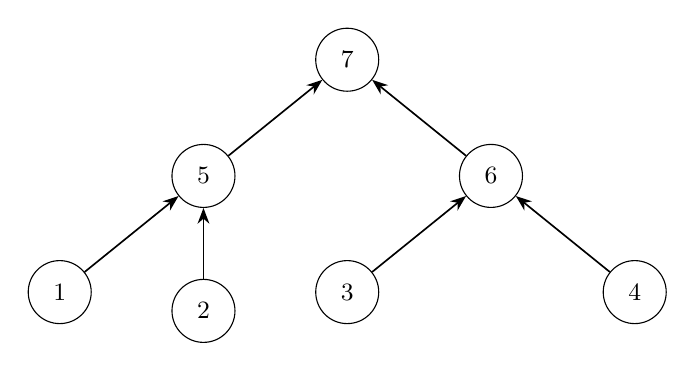
\begin{tikzpicture}[
  node distance=0.9cm and 1.25cm,
  every node/.style={draw,circle,minimum size=8mm,inner sep=0pt,font=\small},
  edge/.style={-{Stealth[length=2mm]},semithick}
]
\node (r) {7};
\node[below left=of r] (a) {5};
\node[below right=of r] (b) {6};
\node[below left=of a] (c) {1};
\node[below=of a] (d) {2};
\node[below left=of b] (e) {3};
\node[below right=of b] (f) {4};
\draw[edge] (c)--(a); \draw[edge] (d)--(a);
\draw[edge] (e)--(b); \draw[edge] (f)--(b);
\draw[edge] (a)--(r); \draw[edge] (b)--(r);
\end{tikzpicture}
\caption{消去树中的更新方向：子节点指向父节点。}
\label{fig:elim-tree}
\end{figure}

消去树同时给出两种顺序：数值分解按后序从叶到根处理；使用因子求解时，前代和回代分别沿因子依赖的两个方向进行。位于不同树枝且依赖已经满足的节点彼此独立。

排序、符号分解和数值分解的作用不同：排序确定结构次序；符号分解预测因子非零结构和树依赖；数值分解计算实际因子，并根据数值主元选择修正符号预测。

\section{多波前法}

\subsection{波前矩阵}

对消去树中的一个节点，把本节点可以消去的变量记为 $E$，仍需传递到祖先节点的更新变量记为 $U$。按照 $E,U$ 排列，节点的稠密波前矩阵为

\[
F=
\begin{bmatrix}
F_{EE}&F_{EU}\\
F_{UE}&F_{UU}
\end{bmatrix}.
\]

$E$ 中的变量称为完全求和（fully summed）变量：与这些变量有关的原矩阵项和所有后代更新均已装配到当前波前，因此它们是当前节点的候选消去变量。$U$ 中的信息尚未在当前节点完全求和，只参与更新。

\begin{figure}[htbp]
\centering
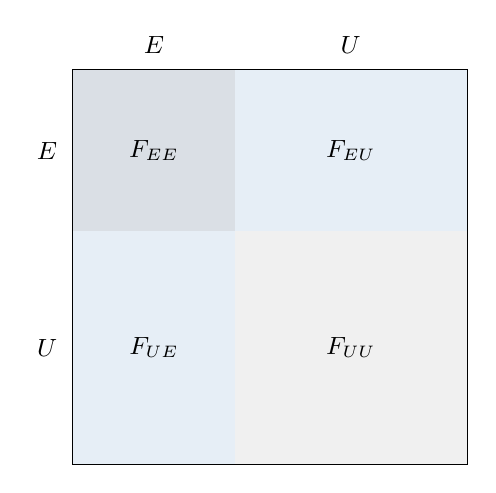
\begin{tikzpicture}[font=\small]
  \draw[thick] (0,0) rectangle (5,5);
  \draw[thick] (2.05,0)--(2.05,5);
  \draw[thick] (0,2.95)--(5,2.95);
  \fill[MumpsBlue!16] (0,2.95) rectangle (2.05,5);
  \fill[MumpsCyan!12] (2.05,2.95) rectangle (5,5);
  \fill[MumpsCyan!12] (0,0) rectangle (2.05,2.95);
  \fill[gray!12] (2.05,0) rectangle (5,2.95);
  \node at (1.025,3.975) {$F_{EE}$};
  \node at (3.525,3.975) {$F_{EU}$};
  \node at (1.025,1.475) {$F_{UE}$};
  \node at (3.525,1.475) {$F_{UU}$};
  \node[above] at (1.025,5.08) {$E$};
  \node[above] at (3.525,5.08) {$U$};
  \node[left] at (-0.08,3.975) {$E$};
  \node[left] at (-0.08,1.475) {$U$};
\end{tikzpicture}
\caption{方形波前矩阵的主元区和更新区。}
\label{fig:frontal-matrix}
\end{figure}

非对称情形消去 $E$ 后得到

\[
P_FFQ_F=
\begin{bmatrix}
L_{EE}&0\\
L_{UE}&I
\end{bmatrix}
\begin{bmatrix}
U_{EE}&U_{EU}\\
0&C
\end{bmatrix},
\]

其中贡献块为

\[
C=F_{UU}-F_{UE}F_{EE}^{-1}F_{EU}.
\]

对称情形相应地写成

\[
P_F^TFP_F=
\begin{bmatrix}
L_{EE}&0\\L_{UE}&I
\end{bmatrix}
\begin{bmatrix}
D_{EE}&0\\0&C
\end{bmatrix}
\begin{bmatrix}
L_{EE}^T&L_{UE}^T\\0&I
\end{bmatrix},
\]

\[
C=F_{UU}-L_{UE}D_{EE}L_{UE}^T.
\]

节点保存已经得到的因子块，并把 $C$ 传给父节点。

\subsection{装配与 extend-add}

当前波前由原矩阵项和子节点贡献块相加得到。设 $F^{(A)}$ 是装配到本节点的原矩阵项，子节点 $c$ 的贡献块为 $C_c$，$R_c$ 把子节点局部变量编号映射到当前波前局部编号，则

\[
F=F^{(A)}+
\sum_{c\in\operatorname{child}(F)}R_c^TC_cR_c.
\]

该操作称为扩展累加（extend-add）。$R_c$ 不要求子节点变量在父波前中连续；它根据全局变量编号完成嵌入和累加。所有子贡献到达后，本节点的完全求和区才完整。

叶节点只装配原矩阵项；内部节点同时装配原矩阵项和子贡献；根节点消去剩余变量，不再向父节点产生贡献块。因而，多波前数值分解可以表示成消去树上的递归：

\[
\operatorname{factor}(v):
\quad
\bigl\{\operatorname{factor}(c)\bigr\}_{c\in\operatorname{child}(v)}
\longrightarrow
\operatorname{assemble}(F_v)
\longrightarrow
\operatorname{eliminate}(F_v)
\longrightarrow C_v.
\]

\subsection{波前规模与运算量}

设一个波前有 $f$ 个总变量，其中 $p$ 个在本节点消去，更新区规模为

\[
u=f-p.
\]

非对称情形需要存储主元列和主元行；其数量级为

\[
p(2f-p).
\]

对称情形只需存储一个三角部分，对应数量级为

\[
pf.
\]

数值工作由主元块分解、块行/块列求解和 Schur 补更新组成。当 $f\gg p$ 时，主要计算来自 $p\times u$ 与 $u\times p$ 形成的尾部更新；当 $p$ 较大时，主元块自身的稠密分解也占据主要部分。

\section{超节点法}

\subsection{超节点的定义}

以列式因子 $L$ 为例，若一组连续列

\[
J=\{s,s+1,\ldots,t\}
\]

在对角块以下具有相同的非零行结构，则这些列可以组成一个超节点。设公共行集为 $R$，超节点在 $L$ 中的数值部分写成

\[
L_{J\cup R,J}=
\begin{bmatrix}
L_{JJ}\\
L_{RJ}
\end{bmatrix},
\]

其中 $L_{JJ}$ 是稠密下三角块，$L_{RJ}$ 是稠密矩形块。

\begin{figure}[htbp]
\centering
\begin{tikzpicture}[x=0.48cm,y=0.48cm,font=\small]
  \draw[thick] (0,0) rectangle (10,10);
  \foreach \x in {1,...,9} {\draw[gray!18] (\x,0)--(\x,10);}
  \foreach \y in {1,...,9} {\draw[gray!18] (0,\y)--(10,\y);}
  \fill[MumpsBlue!22] (2,6) rectangle (5,9);
  \fill[MumpsCyan!20] (2,2) rectangle (5,6);
  \draw[MumpsBlue,very thick] (2,2) rectangle (5,9);
  \node at (3.5,7.5) {$L_{JJ}$};
  \node at (3.5,4) {$L_{RJ}$};
  \node[above,MumpsBlue] at (3.5,10.15) {连续列 $J$};
  \draw[decorate,decoration={brace,amplitude=4pt},MumpsCyan]
    (5.25,2)--(5.25,6) node[midway,right=5pt] {公共行集 $R$};
\end{tikzpicture}
\caption{超节点的连续列及其公共非零行结构。}
\label{fig:supernode-structure}
\end{figure}

严格超节点要求列结构完全一致。实际算法还可以把结构接近的相邻列合并为松弛超节点，合并后显式保存由此产生的少量结构零。基本超节点由符号因子的精确结构确定；松弛合并在基本超节点之上进行\cite{demmel1999}。

\subsection{超节点分解公式}

在 Cholesky 或 $LDL^T$ 分解中，设前面超节点对当前列块 $J$ 的更新已经累加，当前块写成

\[
\begin{bmatrix}
A_{JJ}^{(k)}\\
A_{RJ}^{(k)}
\end{bmatrix}.
\]

Cholesky 情形先计算

\[
L_{JJ}L_{JJ}^T=A_{JJ}^{(k)},
\]

再进行三角求解

\[
L_{RJ}=A_{RJ}^{(k)}L_{JJ}^{-T},
\]

随后对尚未分解部分施加块更新

\[
A_{RR}^{(k+1)}=A_{RR}^{(k)}-L_{RJ}L_{RJ}^T.
\]

一般对称不定情形写为

\[
A_{JJ}^{(k)}=L_{JJ}D_{JJ}L_{JJ}^T,
\]

\[
L_{RJ}=A_{RJ}^{(k)}L_{JJ}^{-T}D_{JJ}^{-1},
\]

\[
A_{RR}^{(k+1)}=A_{RR}^{(k)}-L_{RJ}D_{JJ}L_{RJ}^T.
\]

一般非对称超节点 LU 使用行超节点和列超节点形成面板。其块公式为

\[
\begin{bmatrix}
A_{JJ}&A_{JK}\\
A_{KJ}&A_{KK}
\end{bmatrix}
=
\begin{bmatrix}
L_{JJ}&0\\L_{KJ}&I
\end{bmatrix}
\begin{bmatrix}
U_{JJ}&U_{JK}\\0&S_{KK}
\end{bmatrix},
\]

\[
U_{JK}=L_{JJ}^{-1}A_{JK},\qquad
L_{KJ}=A_{KJ}U_{JJ}^{-1},
\]

\[
S_{KK}=A_{KK}-L_{KJ}U_{JK}.
\]

这些公式把一组列的标量更新合并为三角求解和矩阵乘法。

\subsection{左看、右看与上看组织}

超节点分解可以按更新的产生和使用次序分类。

\begin{itemize}
  \item 左看：处理当前超节点时，收集所有以前超节点对它的更新，然后分解当前块；
  \item 右看：一个超节点分解完成后，立即把它的更新散布到所有后续相关超节点；
  \item 上看：按当前列或列块遍历因子结构，沿依赖索引寻找并累加以前列块的贡献。
\end{itemize}

三种组织使用相同的块分解恒等式，区别在于 Schur 补更新何时形成、存放在哪里以及何时累加到目标列块。

\section{多波前法与超节点法的对应关系}

两类方法都建立在排序后的消元结构上，也都用连续或相关的变量集合形成稠密块。它们的主要对应关系见\cref{tab:mf-sn}。

\begin{table}[htbp]
\centering
\caption{多波前法与超节点法的数学组织}
\label{tab:mf-sn}
\begin{tabularx}{\textwidth}{p{0.18\textwidth}XX}
\toprule
项目 & 多波前法 & 超节点法 \\
\midrule
基本单位 & 消去树节点的波前矩阵 & 具有共同列结构的连续列块 \\
子问题输入 & 原矩阵项和子节点贡献块 & 以前超节点对当前列块的更新 \\
中间结果 & 显式贡献块 $C$ & 对后续超节点的块更新 \\
结构索引 & 波前变量列表和父子关系 & 超节点列区间及其行结构 \\
稠密计算 & 波前主元块分解与 Schur 补更新 & 对角块分解、TRSM 和块更新 \\
依赖表示 & 波前消去树 & 超节点消去树或列依赖图 \\
\bottomrule
\end{tabularx}
\end{table}

若把一个超节点及其尚未消去的更新行装配成方形局部矩阵，就得到与波前矩阵相同的 $E/U$ 分块；若把一个波前中连续且结构一致的主元列作为列块，则其主元计算又具有超节点形式。因此，两者的 Schur 补代数相同，差别主要在于稀疏数据如何分组和更新如何组织。

\section{从分解到求解}

分解得到因子后，一般非对称系统按

\[
y=L^{-1}Pb,\qquad x=Q\,U^{-1}y
\]

求解；对称系统按

\[
y=L^{-1}P^Tb,\qquad z=D^{-1}y,
\qquad x=P\,L^{-T}z
\]

求解。多波前表示按消去树节点访问因子块，超节点表示按超节点列块访问因子。多个右端项时，标量或向量三角更新变成块三角求解和矩阵乘法。

\chapter{MUMPS 延迟主元}

本章只讨论 MUMPS 5.6.2 自身采用的数值选主元与延迟主元机制，所有阈值、判据和运行时计数均以 MUMPS 用户手册及数值分解源码为准。

\section{MUMPS 为什么需要延迟主元}

MUMPS 的分析阶段根据矩阵的非零结构建立消元树，并预测每个节点应当消去的变量、波前矩阵规模、因子存储量和计算量。这些预测只包含结构信息，不能保证符号阶段选定的每一个变量在数值分解时都是稳定主元。

设当前节点已经装配出波前矩阵
\[
F=
\begin{bmatrix}
F_{11} & F_{12}\\
F_{21} & F_{22}
\end{bmatrix}.
\]
其中 $F_{11}$ 对应 Fully Summed 变量。这些变量已经收齐所有子节点贡献，因而只有它们能够在当前节点中作为候选主元。$F_{22}$ 所对应的变量尚未完全装配，只能参加更新，不能提前作为当前节点的主元。

如果候选主元相对于所在行或列的其他元素过小，直接消去会产生很大的乘子，放大舍入误差。MUMPS 因而在 Fully Summed 候选区内实施阈值选主元：

\begin{enumerate}
  \item 搜索满足稳定性阈值的 $1\times1$ 主元；
  \item 对称不定问题还可以搜索满足阈值的 $2\times2$ 主元块；
  \item 只有通过数值检验的候选量才在当前节点消去；
  \item 当候选区中不再存在合格主元时，尚未消去的 Fully Summed 变量随贡献块传到父节点。
\end{enumerate}

这些未在原节点消去、而是在父节点重新参加选主元的变量，就是延迟主元。延迟并不表示丢弃变量，也不表示立即把小主元改成零；它只是推迟该变量的消去位置。

\section{MUMPS 的相对阈值 \code{CNTL(1)}}

\subsection{部分阈值选主元}

MUMPS 用 \code{CNTL(1)} 设置数值选主元的相对阈值。记
\[
u=\code{CNTL(1)},\qquad 0\le u\le1.
\]
以非对称矩阵的列搜索形式为例，在高斯消去第 $i$ 步，令
\[
m_i=\max_{k=i,\ldots,n}|a_{ki}|.
\]
只有当候选对角主元满足
\begin{equation}
\boxed{|a_{ii}|\ge u,m_i}
\label{eq:mumps-ptp}
\end{equation}
时，MUMPS 才允许直接接受该主元。MUMPS 也可以按行实施等价的阈值搜索；在多波前实现中，搜索范围被限制在当前波前已经完整装配的候选区域内\cite{mumpsguide}。

式~\eqref{eq:mumps-ptp} 比较的是候选主元与其当前行或列最大元素，而不是与整个活动子矩阵的最大元素比较。该判据允许消去乘子的模受到 $1/u$ 的控制，对应消去步的增长因子上界为 $1+1/u$\cite{mumpsguide}。

\subsection{参数取值及其含义}

MUMPS 5.6.2 对 \code{CNTL(1)} 的规定如下：

\begin{center}
\begin{tabularx}{0.92\textwidth}{>{\ttfamily}l X}
\toprule
CNTL(1) & 数值含义 \\
\midrule
$<0$ & 按 $0$ 处理。\\
$=0$ & 不进行数值选主元；遇到零主元时分解失败，除非另有静态主元或零主元处理机制介入。\\
$>0$ & 启用阈值数值选主元。\\
$>1$，非对称 & 按 $1$ 处理。\\
$>0.5$，对称 & 按 $0.5$ 处理。\\
\bottomrule
\end{tabularx}
\end{center}

默认值为
\[
u=
\begin{cases}
0.01, & \text{非对称矩阵或一般对称矩阵},\\
0,    & \text{对称正定矩阵}.
\end{cases}
\]
对于对角占优并且不需要数值选主元的矩阵，可以令 $u=0$ 以减少分解时间。对于一般不定问题，增大 $u$ 会提高接受主元的要求，通常有利于数值稳定性，但也会增加换主元、延迟主元、填充以及额外计算。常见的阈值选择为 $0.01$ 或 $0.1$\cite{mumpsguide}。

\begin{keypoint}
在 MUMPS 中，控制延迟主元发生概率的主要相对阈值是 \code{CNTL(1)}。$u$ 越大，判据越严格，候选变量越可能被推迟；$u$ 越小，越倾向于维持分析阶段预测的消去顺序。
\end{keypoint}

\section{非对称 LU 分解的主元判定}

\subsection{在 Fully Summed 区内搜索}

非对称情形计算带行、列置换的 LU 分解。设当前波前中可尝试消去的 Fully Summed 变量数为 \code{NASS}，已经成功消去的主元数为 \code{NPIV}，则下一个主元位置为
\[
i=\code{NPIV}+1.
\]
MUMPS 不会只检查位置 $i$ 的对角元。它在剩余 Fully Summed 候选中轮流检查可用的主元行或列，并允许把合格候选交换到第 $i$ 个位置。更新变量虽然不能被选作主元，但其中的元素仍参与行或列最大值的计算，因为它们决定消去乘子的大小。

对某个候选主元 $p$，记 $r_{\max}$ 为该候选相关行或列在当前有效范围内的最大元素模。MUMPS 源码中的核心相对检验是
\begin{equation}
|p|\ge u,r_{\max}.
\label{eq:mumps-lu-relative}
\end{equation}
此外还必须通过绝对小量保护：
\begin{equation}
|p|>max\{s_{\mathrm{abs}},\operatorname{tiny}(r_{\max})\}.
\label{eq:mumps-lu-absolute}
\end{equation}
这里 $s_{\mathrm{abs}}$ 是当前运行模式下的绝对小主元界；\code{tiny} 是浮点数可表示范围的保护量。式~\eqref{eq:mumps-lu-relative} 是由 \code{CNTL(1)} 控制的主要稳定性判据，式~\eqref{eq:mumps-lu-absolute} 用于防止零主元、极小主元和下溢。

MUMPS 对候选的处理可概括为：

\begin{enumerate}
  \item 若当前位置的候选满足相对阈值和绝对阈值，直接接受；
  \item 否则在剩余 Fully Summed 候选中寻找满足相同条件的行内或列内最大元素；
  \item 找到后执行相应置换，把它移到当前主元位置；
  \item 接受主元、更新因子与剩余子矩阵，并令 \code{NPIV} 加一；
  \item 若遍历候选区后仍没有合格主元，则停止当前波前的继续消去。
\end{enumerate}

因此，“某个预定对角元不满足式~\eqref{eq:mumps-lu-relative}”并不等于立刻延迟。只有当当前 Fully Summed 区中找不到任何可接受的替代主元时，尚未消去的变量才整体留到贡献块中。

\section{对称不定 $LDL^{T}$ 分解的主元判定}

\subsection{$1\times1$ 主元}

为了保持对称性，MUMPS 对行和列实施相同置换，并计算
\[
P^{T}AP=LDL^{T},
\]
其中 $D$ 可以含有 $1\times1$ 和 $2\times2$ 对角块。

对于 $1\times1$ 候选 $p$，源码分别统计候选在当前 Fully Summed 区和相关更新区中的最大元素尺度，记为 $a_{\max}$ 与 $r_{\max}$。接受条件为
\begin{equation}
\boxed{
|p|\ge u\max\{a_{\max},r_{\max}\}
}
\label{eq:mumps-ldlt-1x1-rel}
\end{equation}
并同时要求
\begin{equation}
|p|>max\{s_{\mathrm{abs}},\operatorname{tiny}(r_{\max})\}.
\label{eq:mumps-ldlt-1x1-abs}
\end{equation}
如果当前候选不满足 $1\times1$ 判据，MUMPS 会寻找与它耦合较强的另一个 Fully Summed 变量，尝试构造 $2\times2$ 主元块。该主元块继续由相对阈值 $u=\code{CNTL(1)}$ 控制，并通过对逆主元块所产生消去乘子的估计进行检验。

\subsection{$2\times2$ 主元块}

设候选主元块为
\[
D_p=
\begin{bmatrix}
a & b\\
b & c
\end{bmatrix},qquad
\Delta=ac-b^2.
\]
若 $\Delta=0$，主元块奇异，不能接受。因为
\[
D_p^{-1}
=\frac{1}{\Delta}
\begin{bmatrix}
c & -b\\
-b & a
\end{bmatrix},
\]
MUMPS 直接根据 $D_p^{-1}$ 作用于其余行时可能产生的乘子大小建立检验。记 $r_{\max}$、$t_{\max}$ 分别为两个候选变量与剩余有效区域耦合元素的最大模，$a_{\max}$ 为搜索第二个候选时得到的耦合尺度。源码要求
\begin{align}
u\bigl(|c|r_{\max}+a_{\max}t_{\max}\bigr)
  &\le |\Delta|,\label{eq:mumps-2x2-a}\\
u\bigl(|a|t_{\max}+a_{\max}r_{\max}\bigr)
  &\le |\Delta|.\label{eq:mumps-2x2-b}
\end{align}
当启用了非零的绝对小主元界时，还要求
\begin{equation}
\sqrt{|\Delta|}>s_{\mathrm{abs}}.
\label{eq:mumps-2x2-abs}
\end{equation}
这些条件共同限制 $D_p^{-1}$ 产生的两个消去乘子。若全部满足，MUMPS 接受该 $2\times2$ 块，执行对称置换，并令 \code{NPIV} 增加 2；否则继续检查其他候选。所有允许的 $1\times1$ 和 $2\times2$ 候选都失败后，剩余变量才延迟。

\section{延迟量怎样形成并传到父节点}

\subsection{三个运行时计数}

延迟主元在 MUMPS 中由三个运行时整数直接刻画：
\[
\begin{aligned}
\code{NASS}&: &&\text{当前波前中允许尝试消去的 Fully Summed 变量数},\\
\code{NPIV}&: &&\text{实际通过主元检验并已消去的变量数},\\
\code{NELIM}&: &&\text{未在当前节点消去的变量数}.
\end{aligned}
\]
节点分解结束后，MUMPS 计算
\begin{equation}
\boxed{
\code{NELIM}=\code{NASS}-\code{NPIV}
}.
\label{eq:mumps-nelim}
\end{equation}
\code{NELIM} 不是分析阶段预先确定的常量，而是由实际数值和选主元结果决定的运行时量。

若 \code{NPIV=NASS}，所有候选变量均在当前节点成功消去；若 \code{NPIV<NASS}，则贡献块的变量排列可抽象为
\[
\underbrace{\code{NASS}-\code{NPIV}}_{\text{延迟变量}}
\quad+\quad
\underbrace{\code{NFRONT}-\code{NASS}}_{\text{原有更新变量}}.
\]
因此贡献块不再只是符号分析预测的 Schur 补变量，还在其前部携带实际延迟变量及相应的全局行、列索引。

\subsection{父节点重新装配}

子节点完成后，贡献块留在本地栈中或通过 MPI 发送给父节点的 owner 进程。父节点读取子节点实际返回的 \code{NELIM}，把这些变量加入自己的 Fully Summed 候选集合。其可尝试消去的变量数因此包含
\[
\code{NASS}_{p}
=\code{NASS}_{p}^{\mathrm{symbolic}}
+\sum_{c\in\operatorname{child}(p)}\code{NELIM}_{c}.
\]
父节点随后根据新的实际规模建立波前、执行 extend-add，并对这些变量重新进行阈值选主元。延迟变量在父节点处已经收到了更多子树贡献，数值环境发生变化，因而可能在新的候选集合中找到可接受主元。

整个过程可以写成
\begin{align*}
\text{子节点找不到合格主元}
&\longrightarrow \code{NPIV}<\code{NASS}
\longrightarrow \code{NELIM}>0,\\
&\longrightarrow \text{并入贡献块}
\longrightarrow \text{父节点重新装配和选主元}.
\end{align*}

若这种延迟一直传播到消元树根，而根节点仍存在 \code{NASS}\,$\ne$\,\code{NPIV}，则已经没有更高层节点可以接收这些变量。在普通分解路径中，这将导致零主元或奇异性错误。需要处理秩亏矩阵时，应显式启用 MUMPS 的零主元行检测机制。

\section{静态主元、延迟主元与零主元检测}

\subsection{静态主元 \code{CNTL(4)}}

MUMPS 可以用静态主元减少数值延迟带来的结构增长。静态主元阈值由实数参数 \code{CNTL(4)} 控制：

\begin{center}
\begin{tabularx}{0.92\textwidth}{>{\ttfamily}l X}
\toprule
CNTL(4) & 处理方式 \\
\midrule
$<0$ & 不启用静态主元；默认值为 $-1$。\\
$=0$ & 启用自动阈值，当前版本取 $\sqrt{\epsilon}\,\|A_{\mathrm{pre}}\|$。\\
$>0$ & 启用静态主元，模小于 \code{CNTL(4)} 的主元被替换为该阈值，并保留原符号。\\
\bottomrule
\end{tabularx}
\end{center}

其中 $A_{\mathrm{pre}}$ 是经过置换和缩放后的待分解矩阵，$\epsilon$ 是机器精度。MUMPS 在运行时把 \code{CNTL(1)} 控制的数值选主元与 \code{CNTL(4)} 控制的静态主元结合起来：本来会因部分阈值选主元而推迟的小主元，可以通过受控扰动留在预定消去位置，从而避免父节点波前继续膨胀。被修改的主元总数由 \code{INFOG(25)} 返回\cite{mumpsguide}。

静态主元改变了原矩阵的数值，因此通常需要在求解后进行迭代改进。它与延迟主元的区别是：

\begin{itemize}
  \item 延迟主元不修改主元数值，而是改变变量实际消去的节点；
  \item 静态主元尽量维持符号阶段的消去位置，但会扰动过小主元；
  \item 前者增加动态填充和内存不确定性，后者把这部分代价转换为数值扰动及后处理代价。
\end{itemize}

需要特别注意：\code{CNTL(4)} 是静态主元阈值，而 \code{ICNTL(4)} 只是控制错误、警告和诊断信息的输出级别，两者没有相同的算法含义。

\subsection{零主元行检测}

\code{ICNTL(24)=1} 启用零主元行检测。其判定尺度由 \code{CNTL(3)} 给出。记阈值为 $t_{\mathrm{null}}$，则
\[
t_{\mathrm{null}}=
\begin{cases}
\code{CNTL(3)}\,\|A_{\mathrm{pre}}\|, & \code{CNTL(3)}>0,\\
\epsilon\,\|A_{\mathrm{pre}}\|\sqrt{N_h}, & \code{CNTL(3)}=0,\\
|\code{CNTL(3)}|, & \code{CNTL(3)}<0,
\end{cases}
\]
其中 $N_h$ 是消元树最深分支上的变量数。当候选行或列的无穷范数小于该阈值时，MUMPS 将其识别为零主元行。该功能用于估计秩亏并支持奇异系统求解或零空间基的计算，它不是普通延迟主元判据。

静态主元与零主元检测不兼容；当 \code{ICNTL(24)=1} 时，静态主元选项会被忽略。若根节点由 ScaLAPACK 分解，根上的零主元检测能力还会受到限制；需要精确检测时可令 \code{ICNTL(13)=1}，使根节点采用顺序分解路径，但这可能降低性能\cite{mumpsguide}。

\section{延迟主元对 MUMPS 数值分解的影响}

延迟主元发生后，实际分解与分析阶段的结构预测产生偏差，主要体现在以下方面：

\begin{enumerate}
  \item \textbf{波前扩大。} 延迟变量进入父节点的 Fully Summed 区，使父节点的实际波前大于符号预测。
  \item \textbf{额外填充。} 延迟变量与父节点原有变量建立新的耦合，产生分析阶段未预测的因子非零元。
  \item \textbf{计算量增加。} 父节点需要在更大的稠密波前上装配、搜索主元并更新 Schur 补。
  \item \textbf{内存需求增加。} 贡献块和父节点波前同时增大，分析阶段的内存估计可能不足，因此 \code{ICNTL(14)} 提供额外工作空间比例，\code{ICNTL(23)} 可以设置每个进程的内存上限。
  \item \textbf{并行负载偏移。} 节点与 MPI 进程的映射在分析阶段已经确定，延迟造成的新增工作仍沿既定消元树和候选进程集合执行，不会把普通节点任意迁移到全局空闲进程。
\end{enumerate}

\begin{keypoint}
MUMPS 延迟主元的完整判定链是：使用 \code{CNTL(1)} 在 Fully Summed 候选区内搜索满足部分阈值条件的 $1\times1$ 主元；对称不定问题还按同一个 $u$ 检查 $2\times2$ 主元块；若所有允许候选均失败，则 \code{NPIV} 停止增长，并以 \code{NELIM=NASS-NPIV} 的形式把变量随贡献块传给父节点。\code{CNTL(4)} 的静态主元和 \code{ICNTL(24)} 的零主元检测是与这一过程相关、但含义不同的两套机制。
\end{keypoint}

\chapter{MUMPS 并行策略与内存管理}

MUMPS 采用异步多波前并行方法。分析阶段建立消去树映射、节点 owner 和大型节点的候选进程集合；数值分解阶段依据依赖满足情况、消息到达顺序和受限的运行时负载信息调度任务。因此，其并行组织是静态映射与动态任务调度的结合，而不是完全静态的层同步，也不是允许任意进程接管任意节点的全局工作窃取\cite{mumpsguide,amestoy2001,amestoy2006}。

\section{进程、线程与数据分布}

\subsection{MPI 工作进程}

MUMPS 初始化时已经知道 MPI 通信域大小和 \code{PAR}。若 \code{PAR=1}，host rank 同时是工作进程；若 \code{PAR=0}，host 不承担数值工作，其余 rank 组成工作通信域。内部量 \code{NSLAVES} 或 \code{SLAVEF} 表示工作进程数。该数量在区分 Type 1 和 Type 2 节点之前已经确定，因此节点分类不参与决定 MPI 进程总数。

master、slave、owner 和 candidate 都是 MPI rank 在特定任务中的角色，不等同于物理计算节点。一台机器上可以运行多个 MPI rank，一个 rank 在不同波前中也可以承担不同角色。

\subsection{三类并行来源}

MUMPS 中可以同时出现三类并行：

\begin{enumerate}
  \item 消去树并行：不同 MPI 进程同时处理不同树枝上的波前；
  \item 波前内部 MPI 并行：一个大型 Type 2 波前由一个 master 和若干参与进程协同处理；
  \item MPI 进程内部线程并行：多线程 BLAS 以及 MUMPS 的部分 OpenMP 区域在同一 rank 的共享地址空间中执行。
\end{enumerate}

第一、二项是 MPI 进程间并行，第三项是进程内共享内存并行。混合版本的线程并行主要来自多线程 BLAS，同时包含若干由 OpenMP 实现的并行区域\cite{mumpsguide}。

\section{分析阶段的节点代价}

\subsection{单个波前的规模}

在 \src{mumps\_static\_mapping.F} 中，\src{MUMPS\_TREECOSTS} 对节点 \code{pos} 取得

\[
p=\code{npiv},\qquad f=\code{nfront},
\]

其中 $p$ 是节点计划消去的变量数，$f$ 是波前总阶数，贡献块的预测阶数为

\[
c=f-p.
\]

调用

\begin{lstlisting}[language=Fortran]
CALL MUMPS_CALCNODECOSTS(
    npiv,
    nfront,
    cv_ncostw(pos),
    cv_ncostm(pos))
\end{lstlisting}

后，\code{cv\_ncostw(pos)} 保存该节点的计算量估计，\code{cv\_ncostm(pos)} 保存该节点的因子存储量估计。这里的“计算量”是稠密主元块分解、三角求解和 Schur 补更新的浮点运算估计；“因子存储量”是该节点预计保留的因子数值个数，不是进程已经申请的字节数。

MUMPS 5.6.2 的普通非低秩路径使用以下公式。一般非对称矩阵为

\[
\begin{aligned}
W_v={}&2fp(f-p-1)
+\frac{p(p+1)(2p+1)}{3}
+\frac{(2f-p-1)p}{2},\\
M_v={}&p(2f-p).
\end{aligned}
\]

对称矩阵为

\[
\begin{aligned}
W_v={}&p\left[
f^2+2f-(f+1)(p+1)
+\frac{(p+1)(2p+1)}{6}
\right],\\
M_v={}&pf.
\end{aligned}
\]

实现将 $W_v,M_v$ 分别存入 \code{cv\_ncostw} 和 \code{cv\_ncostm}。这两个数用于分析阶段的相对负载比较和节点映射\cite{mumpssource}。

\subsection{子树累计代价}

\src{MUMPS\_TREECOSTS} 递归遍历实际子节点，定义

\[
T^W_v=W_v+\sum_{c\in\operatorname{child}(v)}T^W_c,
\qquad
T^M_v=M_v+\sum_{c\in\operatorname{child}(v)}T^M_c.
\]

对应数组为 \code{cv\_tcostw(v)} 和 \code{cv\_tcostm(v)}。单节点代价用于普通层中的节点映射；累计代价用于把一个完整的 Level-0 子树作为整体映射。分析阶段使用这些估计更新每个进程的累计工作量

\[
\code{cv\_proc\_workload(proc)}
\]

和累计内存量

\[
\code{cv\_proc\_memused(proc)}.
\]

\section{Level-0 子树映射}

Level-0 不是“树深度等于 0 的所有节点”，也不是“只由一个进程执行的一棵唯一子树”。它是消去树底部的一组互不重叠子树。每棵 Level-0 子树有一个边界根；该根以下的全部后代属于同一子树。

\src{MUMPS\_ROOTLIST} 先从消去树根列表开始，\src{MUMPS\_LAYERL0} 再把当前边界逐步向叶方向展开，形成数量足够、代价可分配的树底子树。因此，构造过程从根列表开始细化，而最终得到的是靠近叶侧的子树划分。

标准路径中的 Level-0 最小候选数量为

\[
\code{MINSIZE\_L0}=3\,\code{SLAVEF}.
\]

内部控制路径还可以取 $6\,\code{SLAVEF}$ 或 $2\,\code{SLAVEF}$。这些值控制映射阶段希望形成的 Level-0 边界规模，不表示每个进程只能获得一棵子树。

\src{MUMPS\_ARRANGEL0} 按子树累计代价调用 \src{MUMPS\_FIND\_BEST\_PROC}：

\[
\text{Level-0 根 }r
\longmapsto
\operatorname*{argmin}_{q\in\mathcal P}
\{\text{当前累计负载或内存}\},
\]

同时受进程可用性和内存约束限制。确定边界根的 owner 后，\src{MUMPS\_MAPSUBTREE} 调用 \src{MUMPS\_MAPBELOW}，递归执行

\[
\code{procnode(descendant)}=
\code{procnode(subtree\_root)}.
\]

例如，若 Level-0 根 $A$ 被映射到 rank 2，则 $A$ 以下的 $B,C,D,E$ 也映射到 rank 2。该子树内部的贡献块在同一 MPI 地址空间中装配；一个 rank 可以拥有多棵 Level-0 子树。

\section{普通层、节点类型与阈值}

\subsection{layernmb}

\code{layernmb} 是静态映射算法中的层编号。它不是 MPI rank，也不是树的数学深度数组。

\code{layernmb=0} 对应 Level-0 子树层；正值表示 Level-0 边界以上依次处理的映射层。

\src{MUMPS\_FIND\_THISLAYER} 产生该层的节点列表，随后执行节点分类、代价处理和进程映射。

\subsection{Type 0 和 Type 1}

多进程情况下，Level-0 边界根被标记为 Type 0，其后代在内部标记为 (-1)，最终继承同一个 owner。只有一个工作进程时，源码把所有节点设为 Type 0。

Level-0 以上不满足 Type 2 条件、且未被指定为特殊 Type 3 的节点被设为 Type 1。Type 1 节点只有一个 owner；该进程负责装配波前、执行主要分解、保存因子并产生贡献块。

\subsection{Type 2 的精确判据}

\src{MUMPS\_ASSIGN\_TYPES} 中，普通层节点成为 Type 2 需要同时满足：

\[
f-p>\code{KEEP(9)},
\]

\[
\code{ICNTL(59)}=0,
\]

并且源码变量 \code{in.ne.0}，即该节点具有实际子节点。

MUMPS 5.6.2 的 \src{MUMPS\_ISTYPE2BYSIZE} 还写有

\begin{lstlisting}[language=Fortran]
((npiv > cv_keep(4)).or.(.TRUE.))
\end{lstlisting}

因此 \code{KEEP(4)} 对 Type 2 判定实际不构成限制。标准默认值为：

\begin{table}[htbp]
\centering
\caption{MUMPS 5.6.2 标准默认节点阈值}
\label{tab:type2-threshold}
\begin{tabular}{lcc}
\toprule
矩阵类别 & \code{KEEP(4)} & \code{KEEP(9)} \\
\midrule
一般非对称 & 32 & 700 \\
对称 & 24 & 400 \\
\bottomrule
\end{tabular}
\end{table}

所以在标准默认值下，Type 2 的有效规模条件是：

\[
\begin{cases}
f-p>700, & \text{一般非对称},\\
f-p>400, & \text{对称},
\end{cases}
\]

再加上“有实际子节点”和“\code{ICNTL(59)=0}”。不满足这些条件的普通节点为 Type 1。内部选项可以修改 \code{KEEP} 值，因此上述数字对应 MUMPS 5.6.2 双精度版本的标准默认设置\cite{mumpssource}。

\subsection{Type 3}

Type 3 不是“消去树根”的同义词。选择过程先在所有满足 \code{FRERE(i)=0} 的结构根中找到预计波前最大的根，记其阶数为 \code{SIZEROOT}。标准自动模式下，只有同时满足以下条件才将该根标记为 Type 3：

\begin{enumerate}
  \item 构建时启用了 ScaLAPACK；
  \item \code{ICNTL(13)=0}，允许并行处理最后的根稠密块；
  \item 工作进程数 \code{SLAVEF}>1；
  \item \code{SIZEROOT}>\code{SLAVEF}；
  \item \code{SIZEROOT}>\code{KEEP(37)}。
\end{enumerate}

默认阈值为

\[
\code{KEEP(37)}=
\max\!\left(800,\left\lfloor70\sqrt{\code{NSLAVES}+1}\right\rfloor\right).
\]

因此，根节点不一定是 Type 3，但 Type 3 一定是所选消去树的结构根。其 \code{procnode} 中仍记录协调进程，而根矩阵和数值计算随后分布到二维 BLACS/ScaLAPACK 进程网格\cite{mumpssource}。

\section{owner 与 Type 1 映射}

这里的“映射”是建立

\[
\text{消去树节点或子树}
\longrightarrow
\text{负责进程及允许参与的进程集合}
\]

的关系。owner 是某个节点的主要负责 rank。对 Type 1，owner 是唯一执行该节点主要数值任务并保存因子的进程；对子节点贡献位于其他 rank 的情况，贡献块通过 MPI 发送到父节点 owner。

\src{MUMPS\_MAP\_LAYER} 先按当前映射目标对节点代价排序，再由 \src{MUMPS\_SORTPROCS} 排列进程。若按浮点工作量平衡，则当前累计工作量小的进程靠前；若按内存平衡，则当前累计内存小的进程靠前；启用优选进程集合时，该集合排在普通进程之前。

对一个 Type 1 节点 $i$，映射器依次检查排序后的进程，选择第一个满足工作量和内存上限的进程 $q$：

\[
\code{cv\_procnode(i)}=q.
\]

随后更新

\[
\code{cv\_proc\_workload(q)}\mathrel{+}=W_i,
\qquad
\code{cv\_proc\_memused(q)}\mathrel{+}=M_i.
\]

这一步使用分析估计，不是对数值分解实际时间和内存的测量。

\section{Type 2 的 owner、候选进程与 CANDIDATES}

Type 2 节点既有一个 master/owner，也有若干候选工作进程。候选数量由 MUMPS 内部的块 2 进程数模型根据 \code{SLAVEF}、矩阵类别、$f$、$f-p$ 以及相关内部控制量计算，不需要先知道节点类型来确定 MPI 总进程数。

分析结束时，所有 Type 2 及分裂链相关节点依次写入

\[
\code{PAR2\_NODES(INIV2)}.
\]

公开数组

\[
\code{CANDIDATES(NSLAVES+1,NB\_NIV2)}
\]

的第 \code{INIV2} 列描述 \code{PAR2\_NODES(INIV2)} 对应节点。若

\[
\code{PAR2\_NODES(3)}=25,
\]

则 \code{INIV2=3} 只表示“第三列候选信息属于节点 25”，不是第三个 MPI rank，也不是第三层。

令

\[
n_c=\code{CANDIDATES(NSLAVES+1,INIV2)}.
\]

前 $n_c$ 项保存主要候选进程的 0-based 工作通信域 rank。例：

\[
\code{CANDIDATES(:,3)}=
[0,2,5,-1,\ldots,3]^T
\]

表示节点 25 的主要候选进程为 rank 0、2、5，最后一项 3 是候选数量。对 Type 2 分裂链，主要候选项之后还可以保存额外参与者；负值标记该扩展列表的结束，解释时需要结合节点的分裂类型。

\src{MUMPS\_RETURN\_CANDIDATES} 把内部候选表复制到 \code{id\%CANDIDATES}。\src{dana\_driver.F} 随后广播 \code{PAR2\_NODES} 和 \code{CANDIDATES}，并在每个 rank 上建立“本 rank 是否为候选”的辅助信息。

Type 2 在数值分解中使用候选集合进行波前内部协作。分析阶段的候选集合并不等于最终实际参与集合。数值分解建立该节点时，根据实际 \code{NFRONT}、贡献块规模、累计负载和内存状态确定 \code{NSLAVES} 及实际进程表。在强制候选约束的路径中，

\[
\{\text{actual slaves}\}\subseteq\{\text{candidate ranks}\};
\]

部分内部策略不强制候选约束，此时选择范围可以扩大到 master 之外的更多工作 rank。无论采用哪条路径，实际进程表一经确定，因子块就按该表分布；随后的前代和回代直接复用实际进程表，不再重新寻找空闲 rank\cite{mumpssource}。

\section{PROCNODE\_STEPS 的含义}

分析阶段把节点顺序转换成数值分解使用的 \code{STEP} 顺序，并生成

\[
\code{id\%PROCNODE\_STEPS(step)}.
\]

该整数不是单纯的 MPI rank。\src{MUMPS\_ENCODE\_PROCNODE} 通过 \src{MUMPS\_ENCODE\_TPN\_IPROC} 把节点类型和 0-based owner rank 编码到同一个整数中。使用时，源码分别通过解码函数取得 owner 或节点类型，例如

\[
\code{MUMPS\_PROCNODE(PROCNODE\_STEPS(step),KEEP(199))}
\]

返回 owner rank。因而 Fortran 表达式

\begin{lstlisting}[language=Fortran]
id%PROCNODE_STEPS(step)
\end{lstlisting}

表示 MUMPS 实例 \code{id} 中第 \code{step} 个数值分解步骤的“类型+owner”编码项；\code{\%} 是 Fortran 派生类型的成员访问符，括号是数组下标。

\section{数值分解阶段的 MPI 组织}

\subsection{初始数据分布}

集中式输入时，矩阵最初位于 host；分布式输入时，各 rank 已持有自己的输入项。分析完成后，MUMPS 根据 \code{PROCNODE\_STEPS} 和波前索引把原矩阵项发送到相应 owner。分解阶段不要求每个 rank 保存完整矩阵；每个 rank 保存映射给自己的矩阵项、波前、贡献块和因子。

\subsection{就绪条件}

每个父节点都有尚未完成的依赖计数 \code{NSTK\_STEPS}。一个子节点完成且其结果在父 owner 上处理后，源码执行

\[
\code{NSTK\_STEPS(STEP(parent))}
\leftarrow
\code{NSTK\_STEPS(STEP(parent))}-1.
\]

当计数变为 0 时，调用 \src{DMUMPS\_INSERT\_POOL\_N} 把父节点插入本地就绪池。这里的“0”表示该父节点需要的所有子贡献均已处理，不表示同一深度的所有节点均已完成。

\subsection{异步主循环}

\src{DMUMPS\_FAC\_PAR} 中，每个工作 rank 在未完成任务存在时交替进行：

\begin{enumerate}
  \item 检查并处理到达的 MPI 消息；
  \item 在没有待处理消息时，从本地就绪池中选择节点；
  \item 装配和分解该节点；
  \item 保存本地因子，把贡献块或控制信息发送给父节点或相关参与进程；
  \item 更新本地负载状态和依赖计数。
\end{enumerate}

不同树枝的 Type 0/1 节点可以同时运行。Type 2 节点由 master 负责主元和任务控制，候选进程处理其持有的面板或更新数据；因而消去树并行与一个大型波前内部的 MPI 并行可以重叠。

分析映射和运行时调度的边界如下：

\begin{itemize}
  \item Type 0/1 节点的 owner 在分析阶段确定，分解阶段仍在该 owner 上处理；
  \item Type 2 的允许参与集合在分析阶段确定，运行时在该集合内进行动态协作；
  \item 本地就绪池在多个已映射到本 rank 的可执行节点之间选择任务；
  \item 消息到达时间和实际负载决定节点何时就绪以及候选进程何时参与。
\end{itemize}

这里的动态性体现在就绪次序、消息推进和 Type 2 实际参与进程的受限选择上；Type 0/1 的 owner 关系仍保持分析阶段的映射结果。

\subsection{Type 0/1：树间并行与进程内计算}

Level-0 子树内部的节点具有同一 owner，子贡献通常直接保留在该 rank 的工作区中；不同 Level-0 子树则可以在不同 rank 上同时推进。一个 rank 可以拥有多棵 Level-0 子树，也可以拥有多个上层 Type 1 节点。

Type 1 节点由唯一 owner 完成装配、主元选择、面板分解、Schur 补更新和因子保存。若父子 owner 不同，子节点将贡献块及其索引发送给父节点 owner。Type 1 的 MPI 并行来自不同 rank 同时处理消去树的不同波前，而不是把单个 Type 1 波前拆分到多个 rank。

\subsection{Type 2：master/slave 波前内部并行}

Type 2 master 在节点真正建立时选择实际 slaves，并记录每个参与进程负责的块行范围。master 负责波前控制、主元选择和主元面板分解；实际 slaves 保存分配给自己的因子或更新块，并接收已分解面板。对第 $k$ 个面板，参与进程并行执行局部更新

\[
C_q\leftarrow C_q-L_qU_k,
\]

其中 $C_q$ 和 $L_q$ 是 rank $q$ 持有的局部块。master 分解后续面板时，其他 rank 可以继续处理前一面板的更新，从而形成面板分解与尾部更新的流水线。候选进程只有在被选入实际 slave 表后才保存相应数据并参加该节点计算。

\subsection{Type 3：二维分布的根波前}

进入 Type 3 根之前，子节点贡献块按照根矩阵的二维块循环分布拆分并发送到相应网格进程，而不是全部集中到协调 rank。各网格进程装配自己的局部根矩阵后，共同建立 ScaLAPACK 描述符并执行并行稠密分解。一般非对称根调用 \code{PDGETRF}，对称正定根调用 \code{PDPOTRF}；未参加根网格的 rank 不持有根矩阵局部块。

三类执行路径构成从树底到树根的并行性转换：树底主要依靠大量独立波前并行，树的中上部依靠 Type 2 波前内部协作，满足条件的根波前使用二维进程网格并行。

\section{延迟主元和估计偏差对调度的影响}

延迟主元使贡献块和祖先波前大于符号估计，因此增加实际浮点运算、通信数据量和进程本地内存。分析阶段已经生成的 owner、Type 2 候选表和树父子关系不会因此整体重做。

若 Type 1 节点因延迟变大，其 owner 不会被普通运行时路径迁移到另一个空闲 rank；该 owner 继续处理实际波前。若 Type 2 节点变大，运行时仍受该节点的实际参与表和所选候选策略约束。强制候选约束时只能从候选表中选择；不强制候选约束的内部路径可以扩大初次选择范围，但并不构成分解过程中的任意工作迁移。

当估计负载与实际负载存在差异时，空闲进程可以执行已经映射到本 rank 的其他就绪子树，在建立 Type 2 节点时被选为实际 slave，或者继续推进通信。此类动态行为不改变 Type 1 的 owner 关系，也不会在求解阶段把未持有因子的空闲 rank 临时加入已有节点。

因此，延迟主元的并行代价包括：父链上的额外计算、较大的贡献块消息、额外装配与内存移动，以及静态估计与实际工作量不一致造成的进程等待。

\section{求解阶段的 MPI 并行}

分解结束后，因子继续分布在生成它们的 rank 上。求解阶段不先把完整 $L,U,D$ 集中到 host，而是沿因子和消去树依赖通信。

\subsection{前代}

一般非对称前代求解

\[
Ly=Pb,
\]

对称情形还要处理 $D$。每个 rank 初始化自己所拥有节点的未完成子依赖计数，并把叶节点加入就绪池。树底不同子树可以同时访问各自保存的因子；一个节点完成局部三角求解和接口变量更新后，将父节点需要的贡献向量发送给父 owner。若父子同属一个 rank，则直接累加到该 rank 的压缩右端项工作区；若 owner 不同，则通过 MPI 发送。父节点在所有子贡献到达后进入就绪池。

Type 2 节点的 master 解出或分发主元相关向量，实际 slaves 使用各自保存的局部因子块并行形成部分更新。通信只传递求解所需的向量和控制信息，不重新传输完整因子。

前代到达 Type 3 根后，右端项按根进程网格的分布方式组织；一般非对称和对称正定路径分别使用 ScaLAPACK 根因子求解例程处理分布式根系统。

\subsection{回代}

回代求解

\[
Ux=y
\quad\text{或}\quad
L^Tx=z.
\]

依赖方向与分解和前代相反：父节点先得到所需解分量，再把子节点更新所需的数据发送给对应 owner；不同树枝收到父级数据后可以并行展开。普通节点只等待父节点提供接口解，不需要再次等待其全部子节点，因此一个父节点完成后可以同时释放多个子树。

Type 2 回代采用“分发--局部更新--归并”方式。master 向实际 slaves 发送接口解，各 slave 用自己的因子块计算部分右端项更新，master 汇总这些更新后完成主元块回代。这里使用的是分解阶段写入节点因子头的实际 slave 表，而不是分析阶段的 \code{CANDIDATES}。

Type 3 根的因子与右端项按二维网格分布，根求解完成后再将所需接口解发送到根以下的节点。一般非对称和对称正定路径分别使用 \code{PDGETRS} 和 \code{PDPOTRS}。

\code{ICNTL(20)} 控制右端项的集中式、稀疏或分布式输入形式，\code{ICNTL(21)} 控制解的集中式或分布式返回。多个右端项使节点局部的向量更新变为矩阵更新，并调用相应的 BLAS-3 核。

求解阶段不再进行主元选择，也不会产生新的延迟主元。数值分解中已经发生的延迟会通过实际因子规模、因子所在 rank 和树上的通信量影响求解。

\section{MPI 进程私有内存与无冲突访问}

MPI rank 具有独立虚拟地址空间。不同 rank 上同名的 Fortran 数组不是同一对象，因此两个进程对各自 \code{A(100)} 的写入不会发生共享内存冲突。跨进程数据只通过 MPI 发送、接收、广播或集合通信转移。

经典分解路径中，每个 rank 主要维护：

\begin{itemize}
  \item 实数或复数工作数组 \code{A}：本地波前、因子、贡献块和数值工作区；
  \item 整数工作数组 \code{IW}：节点头、行列索引、长度、状态和位置描述；
  \item \code{PTRFAC/PTRAST/PTRIST/PTLUST} 等节点位置数组；
  \item MPI 发送与接收缓冲；
  \item 本 rank 所需的右端项和解片段。
\end{itemize}

这些位置量是进程私有 Fortran 数组的下标或偏移，不是跨 MPI rank 有效的共享指针。MUMPS 通常不是为每个节点建立一个独立堆对象，而是在每个 rank 的大工作数组中连续或分区存放多个节点的数据，再通过位置数组定位。

\begin{figure}[htbp]
\centering
\begin{tikzpicture}[font=\small]
  \draw[thick] (0,0) rectangle (11,1.35);
  \fill[MumpsBlue!16] (0,0) rectangle (3.1,1.35);
  \fill[MumpsCyan!15] (3.1,0) rectangle (6.6,1.35);
  \fill[MumpsRed!13] (6.6,0) rectangle (9.2,1.35);
  \fill[gray!15] (9.2,0) rectangle (11,1.35);
  \draw (3.1,0)--(3.1,1.35);
  \draw (6.6,0)--(6.6,1.35);
  \draw (9.2,0)--(9.2,1.35);
  \node at (1.55,0.675) {已保存因子};
  \node at (4.85,0.675) {活动波前与工作区};
  \node at (7.9,0.675) {贡献块};
  \node at (10.1,0.675) {空闲区};
  \draw[decorate,decoration={brace,amplitude=5pt},yshift=3pt]
    (0,1.35)--(11,1.35)
    node[midway,yshift=0.46cm] {单个 MPI rank 的本地数值工作空间示意};
\end{tikzpicture}
\caption{因子、活动数据和贡献块位于各 rank 自己的地址空间。}
\label{fig:local-memory}
\end{figure}

因子和贡献块具有不同生命周期。节点分解完成后，主元块、耦合因子、置换信息和索引一直保留到求解结束；贡献块只用于父节点装配，完成装配后即可释放或复用。父节点不会把子节点因子并入自己的因子区，而只接收子节点的贡献块。全局 $L,U$ 或 $L,D$ 因子由分布在多个 rank 上的节点因子块及其索引共同表示。

\subsection{MPI 发送和接收缓冲}

跨 rank 的贡献块、面板和求解向量必须经过消息缓冲。非阻塞发送返回后，MPI 可能仍在读取发送数据，因此相应缓冲区在请求完成前不能复用。MUMPS 将已打包消息与 \code{MPI\_Request} 一起记录，并通过 \code{MPI\_TEST} 或等价的完成检查确认发送结束；只有请求完成后，该环形缓冲区块才重新进入空闲状态。

接收端先探测消息类型和长度，再把一条消息接收到进程私有缓冲区并解包。普通事件循环一次处理一条接收消息，因此不会由多个 MPI 接收同时覆盖同一缓冲区。由此，进程间的无冲突性来自两个层次：不同 rank 的地址空间彼此隔离；同一 rank 内尚未完成的非阻塞通信缓冲受请求状态保护。

\section{贡献块申请、复用与压缩}

贡献块具有有限生命周期：子节点完成后生成，在父节点装配后可以释放；数值因子通常保留到求解结束。\src{DMUMPS\_ALLOC\_CB} 根据整数描述长度和贡献块数值长度申请本地空间。若当前连续空闲区不足，内存路径可以执行以下操作：

\begin{enumerate}
  \item 使用允许的子节点区域或栈区域进行原位放置；
  \item 回收已经装配完成、不再需要的贡献块；
  \item 移动可移动对象并压缩空洞；
  \item 使用动态贡献块存储路径；
  \item 在仍无法满足请求时返回内存错误。
\end{enumerate}

\code{IPTRLU/LRLU/IWPOS/IWPOSCB/POSFAC} 等变量维护本地工作数组边界、剩余长度和当前因子位置。压缩只修改本 rank 的数组和本地位置记录，不修改其他 MPI rank 的地址。

延迟发生时，实际主元数小于计划主元数，贡献块必须同时保存普通更新变量和延迟变量。\src{DMUMPS\_FAC\_STACK} 根据实际贡献块计算可复用区和移动边界。延迟可能使原位空间不足，从而触发更大的贡献块申请、因子或贡献块移动以及更高的内存高水位。

\section{内存控制与 out-of-core}

主要内存控制参数包括：

\begin{itemize}
  \item \code{ICNTL(14)}：规定数值阶段工作空间相对分析估计的增加百分比；
  \item \code{ICNTL(23)}：规定每个工作进程允许使用的内部工作内存上限，单位为 MB；
  \item \code{ICNTL(22)}：选择 in-core 或 out-of-core 因子存储。
\end{itemize}

当 \code{ICNTL(23)=0} 时，各进程依据分析估计和 \code{ICNTL(14)} 分配工作空间；当其为正数时，MUMPS 在给定的每进程上限内安排整数工作区、实数或复数主工作区、通信缓冲和动态存储。\code{ICNTL(14)} 的默认值随 MPI 进程数而变化，通常在 $20\%$ 至 $35\%$ 之间；单进程对称正定情形的默认值为 $5\%$。数值主元导致额外填充时，可以提高该松弛比例\cite{mumpsguide}。

out-of-core 模式把完整秩数值因子写入各 rank 管理的磁盘文件；求解阶段在使用相应因子时再读取。活动波前、贡献块、通信缓冲和分解工作区仍需要进程私有内存。分析阶段的内存估计用于决定工作数组和数据分布，数值分解后的统计量则反映延迟主元、实际主元和运行时存储路径共同形成的实际使用量。

同一 MPI rank 内启用 OpenMP 时，各线程共享该 rank 的地址空间。共享统计量和池状态由 MUMPS 的线程区域划分及必要的原子/同步操作维护；多线程 BLAS 内部的数据划分由所链接的 BLAS 实现负责。MPI rank 之间则依靠地址空间隔离保证本地工作数组互不冲突。


\appendix
\include{A_延迟主元推广算法}
\chapter{KJI--SAXPY 算法与块分解}

\section{KJI 循环次序}

设 $A\in\mathbb{R}^{n\times n}$ 进行原位 LU 分解，暂不写置换。第 $k$ 步先计算乘子

\[
l_{ik}=\frac{a_{ik}}{a_{kk}},
\qquad i=k+1,\ldots,n,
\]

再更新尾矩阵

\[
a_{ij}\leftarrow a_{ij}-l_{ik}a_{kj},
\qquad i,j=k+1,\ldots,n.
\]

KJI 次序把 $k$ 放在最外层、$j$ 放在中层、$i$ 放在最内层：

\begin{lstlisting}
for k = 1:n-1
    A(k+1:n,k) = A(k+1:n,k) / A(k,k)
    for j = k+1:n
        A(k+1:n,j) = A(k+1:n,j)
                     - A(k,j) * A(k+1:n,k)
    end
end
\end{lstlisting}

固定 $k,j$ 后，内层更新为

\[
A(k+1:n,j)\leftarrow
A(k+1:n,j)-A(k,j)A(k+1:n,k),
\]

即向量形式

\[
y\leftarrow y+\alpha x,
\]

对应 BLAS-1 的 SAXPY；双精度实数对应 DAXPY。列主序存储下，内层 $i$ 遍历同一列的连续元素。

对每个 $k$，全部后续列的更新还可以写成秩一形式

\[
A_{k+1:n,k+1:n}\leftarrow
A_{k+1:n,k+1:n}
-A_{k+1:n,k}A_{k,k+1:n}.
\]

该形式对应 BLAS-2 的 GER。SAXPY 和 GER 表示的是同一消元更新的两种接口组织。将多个秩一更新合并为块更新，是稠密分块 LU 和超节点稀疏分解使用 BLAS-3 的基础\cite{davis2006,demmel1999}。

\section{多个秩一更新的合并}

若连续处理 $b$ 个主元 $k=s,\ldots,s+b-1$，这些主元对后续子矩阵的总更新为

\[
\sum_{q=s}^{s+b-1}l_qu_q^T.
\]

把列向量 $l_q$ 和行向量 $u_q^T$ 分别组合成

\[
L_P=
\begin{bmatrix}l_s&l_{s+1}&\cdots&l_{s+b-1}\end{bmatrix},
\]

\[
U_P=
\begin{bmatrix}
u_s^T\\u_{s+1}^T\\\vdots\\u_{s+b-1}^T
\end{bmatrix},
\]

则

\[
\sum_{q=s}^{s+b-1}l_qu_q^T=L_PU_P.
\]

因此 $b$ 次秩一更新可以合并成一次矩阵乘法：

\[
A_{\mathrm{trail}}\leftarrow
A_{\mathrm{trail}}-L_PU_P.
\]

块分解并不改变 LU 的代数结果；它把重复的向量更新重排为矩阵--矩阵运算。

\section{方形分块 LU}

把当前活动矩阵按宽度 $b$ 分块：

\[
A=
\begin{bmatrix}
A_{11}&A_{12}\\
A_{21}&A_{22}
\end{bmatrix},
\qquad A_{11}\in\mathbb{R}^{b\times b}.
\]

\begin{figure}[htbp]
\centering
\begin{tikzpicture}[font=\small]
  \draw[thick] (0,0) rectangle (5.2,5.2);
  \draw[thick] (2.05,0)--(2.05,5.2);
  \draw[thick] (0,3.15)--(5.2,3.15);
  \fill[MumpsBlue!16] (0,3.15) rectangle (2.05,5.2);
  \fill[MumpsCyan!12] (2.05,3.15) rectangle (5.2,5.2);
  \fill[MumpsCyan!12] (0,0) rectangle (2.05,3.15);
  \fill[gray!12] (2.05,0) rectangle (5.2,3.15);
  \node at (1.025,4.175) {$A_{11}$};
  \node at (3.625,4.175) {$A_{12}$};
  \node at (1.025,1.575) {$A_{21}$};
  \node at (3.625,1.575) {$A_{22}$};
  \draw[MumpsRed,very thick] (0,0)--(0,5.2)--(2.05,5.2)--(2.05,0)--cycle;
  \node[MumpsRed] at (1.025,-0.38) {宽度 $b$ 的面板};
\end{tikzpicture}
\caption{块 LU 的方形活动矩阵和面板。}
\label{fig:kji-block-square}
\end{figure}

块 LU 恒等式为

\[
\begin{bmatrix}
A_{11}&A_{12}\\A_{21}&A_{22}
\end{bmatrix}
=
\begin{bmatrix}
L_{11}&0\\L_{21}&I
\end{bmatrix}
\begin{bmatrix}
U_{11}&U_{12}\\0&S_{22}
\end{bmatrix}.
\]

比较分块乘积得到：

\begin{align}
A_{11}&=L_{11}U_{11},\\
U_{12}&=L_{11}^{-1}A_{12},\\
L_{21}&=A_{21}U_{11}^{-1},\\
S_{22}&=A_{22}-L_{21}U_{12}.
\end{align}

对应一次面板迭代的计算顺序为：

\begin{enumerate}
  \item 在面板中分解主元块 $A_{11}$；
  \item 用左三角求解计算 $U_{12}$；
  \item 用右三角求解计算 $L_{21}$；
  \item 用矩阵乘法更新 $A_{22}$。
\end{enumerate}

第 2、3 步对应 TRSM，第 4 步对应 GEMM。标量 KJI 中连续的 DAXPY/GER 更新由最后一步的 GEMM 集中完成。

\section{主元交换与面板更新}

采用部分选主元时，第 $k$ 列的主元位置为

\[
p_k=\argmax_{i\ge k}|a_{ik}|.
\]

搜索范围是当前列的全部活动行，不限于 $b\times b$ 的对角方块。因此，算法中的“面板”是高为活动行数、宽为 $b$ 的长方形列块；\cref{fig:kji-block-square} 中红色区域表示这一列块。

行交换必须同步作用于当前活动矩阵和已经形成的 $L$ 行，并记录到行置换中。若算法还允许列交换，则活动矩阵的列、全局列编号和列置换必须同步更新，分解关系写成

\[
PAQ=LU.
\]

面板内部不能直接使用尚未包含前面板列贡献的旧数据。设当前面板起点为 $s$，已经接受 $t$ 个主元，准备处理 $k=s+t$ 时，当前列先物化为

\[
A(k:n,k)\leftarrow
A(k:n,k)-L(k:n,s:k-1)U(s:k-1,k).
\]

面板结束后，再把全部已接受列对面板外尾矩阵的贡献一次写回。

\section{延迟主元下的分块 LU}

非对称延迟 LU 算子采用 64 列面板。面板内每一步仍先检查当前列；只有当前列全零时，才按算子规定的活动子块或活动列搜索规则继续选取主元。

若搜索发生在面板尚未完成时，必须先落实该面板已经接受的主元对搜索区域的更新。设面板已经接受 $t\le b$ 列，则写回

\[
A_{\mathrm{trail}}\leftarrow
A_{\mathrm{trail}}-L_P(:,1:t)U_P(1:t,:).
\]

写回后，被检查的活动区是当前 Schur 补。若仍不存在可用主元，则以当前位置为 \code{info}，剩余区间作为延迟后缀。

因此，固定面板宽度 $b$ 是一次最多收集的主元数；遇到延迟时，实际面板宽度可以小于 $b$。

\section{对称块更新}

对称不定分解中，一个面板收集 $1\times1$ 和 $2\times2$ 主元块。设面板乘子为 $L_P$，块对角主元为 $D_P$，尾矩阵更新为

\[
A_{22}\leftarrow A_{22}-L_PD_PL_P^T.
\]

定义

\[
W_P=L_PD_P,
\]

则

\[
A_{22}\leftarrow A_{22}-L_PW_P^T.
\]

分块 Bunch--Kaufman 算子用

\[
S=A_{\mathrm{stored}}-L_PW_P^T
\]

表示面板中尚未写回的 Schur 补。主元测试需要某一列或某一行时，以矩阵--向量乘法计算相应部分；面板完成后，以对称秩二 $k$ 更新写回下三角尾矩阵。面板边界不允许把一个 $2\times2$ 主元拆成两部分。

\section{块三角求解}

块化同样用于因子求解。把下三角系统分块：

\[
\begin{bmatrix}
L_{11}&0\\L_{21}&L_{22}
\end{bmatrix}
\begin{bmatrix}Y_1\\Y_2\end{bmatrix}
=
\begin{bmatrix}B_1\\B_2\end{bmatrix}.
\]

前代为

\[
L_{11}Y_1=B_1,
\]

\[
B_2' = B_2-L_{21}Y_1,
\]

\[
L_{22}Y_2=B_2'.
\]

上三角回代同理。单个右端项时，中间更新是矩阵--向量乘法；多个右端项组成矩阵 $B$ 时，更新

\[
B_2' = B_2-L_{21}Y_1
\]

成为矩阵--矩阵乘法。因而，块因子格式既用于分解阶段合并 SAXPY 更新，也用于求解阶段合并多个右端项的三角更新。

\section{运算量与数据访问}

无论采用标量 KJI 还是块 LU，稠密 $n\times n$ LU 的主导浮点运算量均约为

\[
\frac{2}{3}n^3.
\]

二者的区别是运算组织。标量形式反复读取乘子列和后续列并执行向量更新；块形式把 $b$ 个主元的更新合并，使 $L_P$ 和 $U_P$ 的元素在一次矩阵乘法中重复使用。面板内部仍保留主元搜索、交换和细粒度更新，面板外的主要 Schur 补更新则由 TRSM 和 GEMM 完成。

这一变换可以概括为

\[
\underbrace{\sum_{q=s}^{s+b-1}l_qu_q^T}_{b\text{ 次秩一更新}}
\quad\longrightarrow\quad
\underbrace{L_PU_P}_{\text{一次块更新}}.
\]

\chapter{六阶对称不定矩阵的延迟主元分解示例}

本附录通过一个 $6\times6$ 对称不定矩阵说明延迟主元在多波前分解中的完整传播过程，包括结构排序、消去树构造、波前装配、延迟变量上传、根波前扩展以及 $2\times2$ 主元消去。

\section{原始矩阵与结构排序}

取

\[
\varepsilon=10^{-12},
\qquad
\delta=10^{-14},
\]

并考虑对称矩阵

\[
A=
\begin{bmatrix}
\varepsilon&\delta&1&0&0&0\\
\delta&4&0&1&0&0\\
1&0&0&3&1&0\\
0&1&3&9&0&1\\
0&0&1&0&5&0.5\\
0&0&0&1&0.5&6
\end{bmatrix}.
\]

矩阵的关键特征是

\[
a_{11}=\varepsilon=10^{-12},
\qquad
a_{13}=1.
\]

变量 $x_1$ 的对角元素很小，但它与 $x_3$ 具有较强耦合。删除变量集合 $\{x_3,x_4\}$ 后，结构图分为左右两个子域，因此可将 $\{x_3,x_4\}$ 作为分隔集，并采用排列

\[
p=[x_1,x_2,x_5,x_6,x_3,x_4].
\]

该排列先处理左子域 $\{x_1,x_2\}$ 和右子域 $\{x_5,x_6\}$，最后处理分隔集 $\{x_3,x_4\}$。排列后的矩阵为

\[
P^TAP=
\begin{bmatrix}
\varepsilon&\delta&0&0&1&0\\
\delta&4&0&0&0&1\\
0&0&5&0.5&1&0\\
0&0&0.5&6&0&1\\
1&0&1&0&0&3\\
0&1&0&1&3&9
\end{bmatrix}.
\]

\section{消去树与波前树}

消去 $x_1$ 时，其尚未消去的邻接变量为 $\{x_2,x_3\}$，符号消元产生填充边 $x_2$--$x_3$；消去 $x_5$ 时，其尚未消去的邻接变量为 $\{x_6,x_3\}$，产生填充边 $x_6$--$x_3$。由此得到依赖关系

\[
x_1\longrightarrow x_2\longrightarrow x_3\longrightarrow x_4,
\qquad
x_5\longrightarrow x_6\longrightarrow x_3\longrightarrow x_4.
\]

相应的多波前树可组织为

\begin{figure}[htbp]
\centering
\begin{tikzpicture}[
  font=\small,
  box/.style={draw,thick,rounded corners=2pt,minimum width=3.1cm,minimum height=0.85cm,align=center},
  arr/.style={-{Stealth[length=2.4mm]},thick}
]
  \node[box,fill=MumpsBlue!13] (root) at (0,3.8) {$F_{34}$\\候选变量 $\{x_3,x_4\}$};
  \node[box,fill=MumpsCyan!11] (f2) at (-2.3,2.25) {$F_2$\\候选变量 $\{x_2\}$};
  \node[box,fill=MumpsCyan!11] (f6) at (2.3,2.25) {$F_6$\\候选变量 $\{x_6\}$};
  \node[box] (f1) at (-2.3,0.7) {$F_1$\\候选变量 $\{x_1\}$};
  \node[box] (f5) at (2.3,0.7) {$F_5$\\候选变量 $\{x_5\}$};
  \draw[arr] (f1)--(f2);
  \draw[arr] (f2)--(root);
  \draw[arr] (f5)--(f6);
  \draw[arr] (f6)--(root);
\end{tikzpicture}
\caption{六阶算例的多波前树。贡献块由叶节点向根节点传递。}
\label{fig:six-by-six-front-tree}
\end{figure}

其中根波前 $F_{34}$ 负责分隔集，左右两个分支分别处理两个局部子域。

\section{左侧子树中的主元延迟}

\subsection{$F_1$：$x_1$ 无法作为稳定主元}

叶节点 $F_1$ 的变量顺序为

\[
[\,\underbrace{x_1}_{\text{完全求和变量}}
\mid
\underbrace{x_2,x_3}_{\text{更新变量}}\,],
\]

其波前矩阵为

\[
F_1=
\begin{bmatrix}
\varepsilon&\delta&1\\
\delta&0&0\\
1&0&0
\end{bmatrix}.
\]

设主元接受阈值为 $u=0.1$。对 $x_1$ 检查

\[
|a_{11}|=10^{-12},
\qquad
u\max(|\delta|,1)=0.1.
\]

由于

\[
10^{-12}<0.1,
\]

$x_1$ 不能在 $F_1$ 中作为稳定的 $1\times1$ 主元。该节点没有其他完全求和变量可与之组成 $2\times2$ 主元，因此 $x_1$ 被延迟，随贡献信息传递给父节点 $F_2$。此时

\[
NASS=1,
\qquad
NPIV=0,
\qquad
NELIM=1.
\]

\subsection{$F_2$：消去 $x_2$，继续延迟 $x_1$}

$F_2$ 接收延迟变量 $x_1$ 后，完全求和候选集合由 $\{x_2\}$ 扩展为 $\{x_1,x_2\}$。按

\[
[\,\underbrace{x_1,x_2}_{\text{完全求和变量}}
\mid
\underbrace{x_3,x_4}_{\text{更新变量}}\,]
\]

排列，有

\[
F_2=
\begin{bmatrix}
\varepsilon&\delta&1&0\\
\delta&4&0&1\\
1&0&0&0\\
0&1&0&0
\end{bmatrix}.
\]

$x_1$ 的 $1\times1$ 主元仍不能通过阈值检验。若尝试使用 $\{x_1,x_2\}$ 形成二阶主元块，则

\[
B_{12}=
\begin{bmatrix}
\varepsilon&\delta\\
\delta&4
\end{bmatrix},
\qquad
\det(B_{12})=4\varepsilon-\delta^2
\approx4\times10^{-12}.
\]

该块仍然过于接近奇异，不能作为稳定的 $2\times2$ 主元。相比之下，$x_2$ 满足

\[
4\ge0.1\max(|\delta|,1),
\]

因此采用

\[
D_2=[4]
\]

作为 $1\times1$ 主元，消去 $x_2$，而 $x_1$ 继续延迟。对剩余变量 $[x_1,x_3,x_4]$ 形成的左侧贡献块为

\[
C_{\mathrm{left}}=
\begin{bmatrix}
\varepsilon-\delta^2/4&1&-\delta/4\\
1&0&0\\
-\delta/4&0&-1/4
\end{bmatrix}
\approx
\begin{bmatrix}
10^{-12}&1&0\\
1&0&0\\
0&0&-0.25
\end{bmatrix}.
\]

此时

\[
NASS=2,
\qquad
NPIV=1,
\qquad
NELIM=1.
\]

$x_1$ 已跨过 $F_1$ 和 $F_2$ 两个波前，但仍未被消去。

\section{右侧子树的正常消元}

右侧叶节点 $F_5$ 按 $[x_5\mid x_6,x_3]$ 排列：

\[
F_5=
\begin{bmatrix}
5&0.5&1\\
0.5&0&0\\
1&0&0
\end{bmatrix}.
\]

$x_5$ 可以直接作为主元，取

\[
D_5=[5],
\]

得到变量 $[x_6,x_3]$ 上的贡献块

\[
C_5=
\begin{bmatrix}
-0.05&-0.1\\
-0.1&-0.2
\end{bmatrix}.
\]

父节点 $F_6$ 按 $[x_6\mid x_3,x_4]$ 装配为

\[
F_6=
\begin{bmatrix}
5.95&-0.1&1\\
-0.1&-0.2&0\\
1&0&0
\end{bmatrix}.
\]

$x_6$ 同样可以直接作为 $1\times1$ 主元：

\[
D_6=[5.95].
\]

消去 $x_6$ 后，右侧子树向根节点发送

\[
C_{\mathrm{right}}=
\begin{bmatrix}
-0.20168067&0.01680672\\
0.01680672&-0.16806723
\end{bmatrix},
\]

其变量索引为 $[x_3,x_4]$。右侧子树没有产生延迟主元。

\section{根波前的动态扩展与二阶主元}

根节点原计划只处理分隔集 $\{x_3,x_4\}$。由于左侧子树传来了延迟变量 $x_1$，根节点接收的数据变为

\begin{itemize}
  \item 左侧贡献块：变量集合 $\{x_1,x_3,x_4\}$；
  \item 右侧贡献块：变量集合 $\{x_3,x_4\}$；
  \item 分隔集的原始矩阵块：
  \[
  \begin{bmatrix}
  0&3\\
  3&9
  \end{bmatrix}.
  \]
\end{itemize}

执行扩展累加后，根波前按 $[x_1,x_3,x_4]$ 排列为

\[
F_{34}=
\begin{bmatrix}
10^{-12}&1&-2.5\times10^{-15}\\
1&-0.20168067&3.01680672\\
-2.5\times10^{-15}&3.01680672&8.58193277
\end{bmatrix}.
\]

因此，符号分析预计的 $2\times2$ 根波前在数值阶段扩展为 $3\times3$ 波前。

在根节点中，$x_1$ 的 $1\times1$ 主元仍然失败：

\[
10^{-12}<0.1\times1.
\]

$x_3$ 的对角元素也不足以通过当前检验：

\[
0.20168067<0.1\times3.01680672.
\]

但是变量 $\{x_1,x_3\}$ 可以组成主元块

\[
D_{13}=
\begin{bmatrix}
10^{-12}&1\\
1&-0.20168067
\end{bmatrix},
\qquad
\det(D_{13})\approx-1.
\]

该 $2\times2$ 块非奇异且数值稳定，因此作为一个块主元被接受。延迟变量 $x_1$ 最终与根节点变量 $x_3$ 一同消去。最后剩余的 $x_4$ 形成

\[
D_4\approx[8.58193277].
\]

这个过程说明，小对角元素或零对角元素并不等价于矩阵奇异。当前节点找不到稳定的 $1\times1$ 主元时，可以先延迟变量，在更大的候选集合中寻找稳定的 $2\times2$ 主元。

\section{最终数值主元顺序与分解结果}

符号排序给出的计划顺序为

\[
[x_1,x_2,x_5,x_6,x_3,x_4],
\]

实际数值主元顺序则为

\[
[x_2,x_5,x_6,\{x_1,x_3\},x_4].
\]

令

\[
q=[x_2,x_5,x_6,x_1,x_3,x_4],
\]

$Q$ 为对应的对称置换矩阵，则

\[
Q^TAQ=LDL^T.
\]

各个 $1\times1$ 主元生成的主要消元乘子为

\begin{align*}
L_{x_1,x_2}&=\delta/4=2.5\times10^{-15},
&L_{x_4,x_2}&=1/4=0.25,\\
L_{x_6,x_5}&=0.5/5=0.1,
&L_{x_3,x_5}&=1/5=0.2,\\
L_{x_3,x_6}&=-0.1/5.95=-0.01680672,
&L_{x_4,x_6}&=1/5.95=0.16806723.
\end{align*}

对于根节点的 $2\times2$ 主元，$x_4$ 与 $\{x_1,x_3\}$ 的耦合行为

\[
[r,s]=[-2.5\times10^{-15},\,3.01680672].
\]

因此需要执行块求解

\[
[L_{x_4,x_1},L_{x_4,x_3}]
=[r,s]D_{13}^{-1},
\]

得到

\[
L_{x_4,x_1}\approx3.01680672,
\qquad
L_{x_4,x_3}\approx-3.0193\times10^{-12}.
\]

按照实际数值主元顺序 $q$，最终因子近似为

\[
\resizebox{0.93\textwidth}{!}{$
L=
\begin{bmatrix}
1&0&0&0&0&0\\
0&1&0&0&0&0\\
0&0.1&1&0&0&0\\
2.5\times10^{-15}&0&0&1&0&0\\
0&0.2&-0.01680672&0&1&0\\
0.25&0&0.16806723&3.01680672&-3.0193\times10^{-12}&1
\end{bmatrix}
$},
\]

\[
\resizebox{0.68\textwidth}{!}{$
D=
\begin{bmatrix}
4&0&0&0&0&0\\
0&5&0&0&0&0\\
0&0&5.95&0&0&0\\
0&0&0&10^{-12}&1&0\\
0&0&0&1&-0.20168067&0\\
0&0&0&0&0&8.58193277
\end{bmatrix}
$}.
\]

由于矩阵元素和因子在此处按有限位小数展示，上式是舍入后的分解结果。该算例的核心过程可以概括为

\[
\boxed{
\begin{gathered}
x_1\text{ 在 }F_1\text{ 延迟}
\longrightarrow
x_1\text{ 在 }F_2\text{ 继续延迟}\\
\longrightarrow
F_{34}\text{ 动态扩展}
\longrightarrow
\{x_1,x_3\}\text{ 形成稳定的 }2\times2\text{ 主元}
\end{gathered}}
\]


\backmatter
\renewcommand{\bibname}{参考资料}
\addcontentsline{toc}{chapter}{参考资料}
\begin{thebibliography}{99}
\bibitem{mumpsguide}
MUMPS Consortium. \emph{MUltifrontal Massively Parallel Solver (MUMPS 5.6.2): Users' Guide}, 2023.

\bibitem{mumpssource}
MUMPS Consortium. \emph{MUMPS 5.6.2 Source Distribution}, 2023.

\bibitem{duffreid1983}
I. S. Duff and J. K. Reid. The multifrontal solution of indefinite sparse symmetric linear equations. \emph{ACM Transactions on Mathematical Software}, 9(3):302--325, 1983.

\bibitem{amestoy2001}
P. R. Amestoy, I. S. Duff, J.-Y. L'Excellent, and J. Koster. A fully asynchronous multifrontal solver using distributed dynamic scheduling. \emph{SIAM Journal on Matrix Analysis and Applications}, 23(1):15--41, 2001.

\bibitem{amestoy2006}
P. R. Amestoy, A. Guermouche, J.-Y. L'Excellent, and S. Pralet. Hybrid scheduling for the parallel solution of linear systems. \emph{Parallel Computing}, 32(2):136--156, 2006.

\bibitem{liu1992}
J. W. H. Liu. The multifrontal method for sparse matrix solution: theory and practice. \emph{SIAM Review}, 34(1):82--109, 1992.

\bibitem{demmel1999}
J. W. Demmel, S. C. Eisenstat, J. R. Gilbert, X. S. Li, and J. W. H. Liu. A supernodal approach to sparse partial pivoting. \emph{SIAM Journal on Matrix Analysis and Applications}, 20(3):720--755, 1999.

\bibitem{davis2006}
T. A. Davis. \emph{Direct Methods for Sparse Linear Systems}. SIAM, 2006.

\bibitem{bunchkaufman1977}
J. R. Bunch and L. Kaufman. Some stable methods for calculating inertia and solving symmetric linear systems. \emph{Mathematics of Computation}, 31(137):163--179, 1977.
\end{thebibliography}

\end{document}
